

\chapter{$\Hmuhad$}

\subsection{Misidentified $\Pgt$ lepton background}
The misidentified lepton backgrounds are estimated with full data driven method from the collision data. In $\Hmuhad$ channel, the misidentification $\Pgt$ lepton rate is obtained from independent $\PZ$ + jets data sets and then apply the rate to a control region that orthogonal to the signal region to estimate the misidentified lepton backgrounds.  The control regions for the estimation and validation of the misidentified lepton background are shown in Table.~\ref{tab:fakeratediagram_highmass}. Region I is the signal region with full selection applied. Region III is the background enriched region, in which one or two leptons have loose isolation but not tight isolation. Region II is the same to Region I besides the requirement that $\Pgm$ and $\Pgt$ lepton pairs have the same sign of charge, so as Region IV to Region III. Region III is used to estimate the misidentified background in Region I. Region II and IV are used in the validation of the method. 


\begin{table}[hbt]
 \centering
 {
 \renewcommand{\arraystretch}{1.1}
 \caption{Definition of the samples used to estimate the misidentified lepton background.}
  \label{tab:fakeratediagram_highmass}
  \begin{tabular}{c|c} \hline
\textbf{Region I}              &  \textbf{Region II}             \\ \hline
$\ell^{\pm}_{1}$(isolated)  &  $\ell^{\pm}_{1}$(isolated)             \\
$\ell^{\mp}_{2}$(isolated)  &  $\ell^{\pm}_{2}$(isolated)             \\

\hline \hline
\textbf{Region III}           &  \textbf{Region IV}             \\ \hline
$\ell^{\pm}_{1}$(isolated)  &  $\ell^{\pm}_{1}$(isolated)             \\
$\ell^{\mp}_{2}$(not-isolated )  &  $\ell^{\pm}_{2}$(not-isolated)             \\
\hline
  \end{tabular}
}
\end{table}


%The misidentified lepton backgrounds are estimated with full data driven method from the collision data. In $\Hmuhad$ channel,  the misidentification $\Pgt$ lepton rate is obtained from independent $\PZ$ + jets data sets and then apply the rate to an control region that orthogonal to the signal region to estimate the misidentified lepton backgrounds. This control region is referred as the misidentified lepton estimation region. 

Two sets of Z + jets data sets are used, $\PZ \to \Pgm\Pgm$ and $\PZ\to \Pe \Pe$, to estimate the misidentified lepton rate in order to increase the statistics in the estimation.  In both cases, Z bosons are selected in the invariant mass window $70<M_{ll}<110$ GeV. In $\PZ\to\Pgm\Pgm$, trigger HLT\_IsoMu24 or HLT\_IsoTkMu24 is used. Both muons are required to have $\pt>26$ GeV, $|\eta|<2.4$, cut based tight muon isolation($I^{\Pgm}_{rel}<0.15$) and passing the muon medium ID. In $\PZ\to \Pe \Pe$ case, the trigger HLT\_singleE25eta2p1Tight is used. Both electrons are required to pass $\pt>26$ GeV, $|\eta|<2.1$, cut based tight electron isolation($I^{e}_{rel}<0.1$) and passing MVANonTrigWP80 ID. In the $\PZ$+jets samples, with the selected $\PZ$ boson in an event, the remaining jets are checked if they pass $\Pgt$ ID. The misidentified $\Pgt$ lepton ratio $\Pgt(f_{\Pgt})$ is calculated as in Equation .~\ref{eq:1}, together with one related ratio $f_{\Pgt}$.

\begin{align} 
\Pgm\Pgt(f_{\Pgt})&=\frac{f_{\Pgt}}{1-f_{\Pgt}} \label{eq:1}\\
f_{\Pgt}&=\frac{N_{\Pgt}(\textrm{Z+jets}\ \textrm{tau}\ \textrm{tight}\ \textrm{Iso})}{N_{\Pgt}(\textrm{Z+jets}\ \textrm{tau}\ \textrm{very}\ \textrm{loose}\ \textrm{Iso})} \label{eq:2}
\end{align}



$f_{\Pgt}$ is the ratio between number of jets that pass tight $\Pgt$ MVA isolation ID and number of jets that pass very loose $\Pgt$ MVA isolation ID. The contribution from Diboson sample are subtracted with MC samples, in which the third \Pgt are genuine leptons. With the ratio $f_{\Pgt}$ , misidentified rate $\Pgt(f_{\Pgt})$(Equation.~\ref{eq:2}) is applied as a weight to Region III, which is defined in the same criteria as the signal region, besides $\Pgt$ leptons are required to pass very loose isolation and not pass the tight isolation. The misidentified $\Pgt$ lepton rate $\Pgt(f_{\Pgt})$ shows dependence on tau $\eta$ and tau decay mode, thus $\Pgt(f_{\Pgt})$ is applied in term of tau $\eta$ and tau decay modes. The distribution of $f_{\Pgt}$ is shown in Fig.~ \ref{fig:fakerationumber}, which shows a comparison of the estimated $f_{\Pgt}$ between data and simulated Z+jets samples. 

\begin{figure}[htbp] 
     \centering
     \subfigure[tau decay mode 0 EB]{ 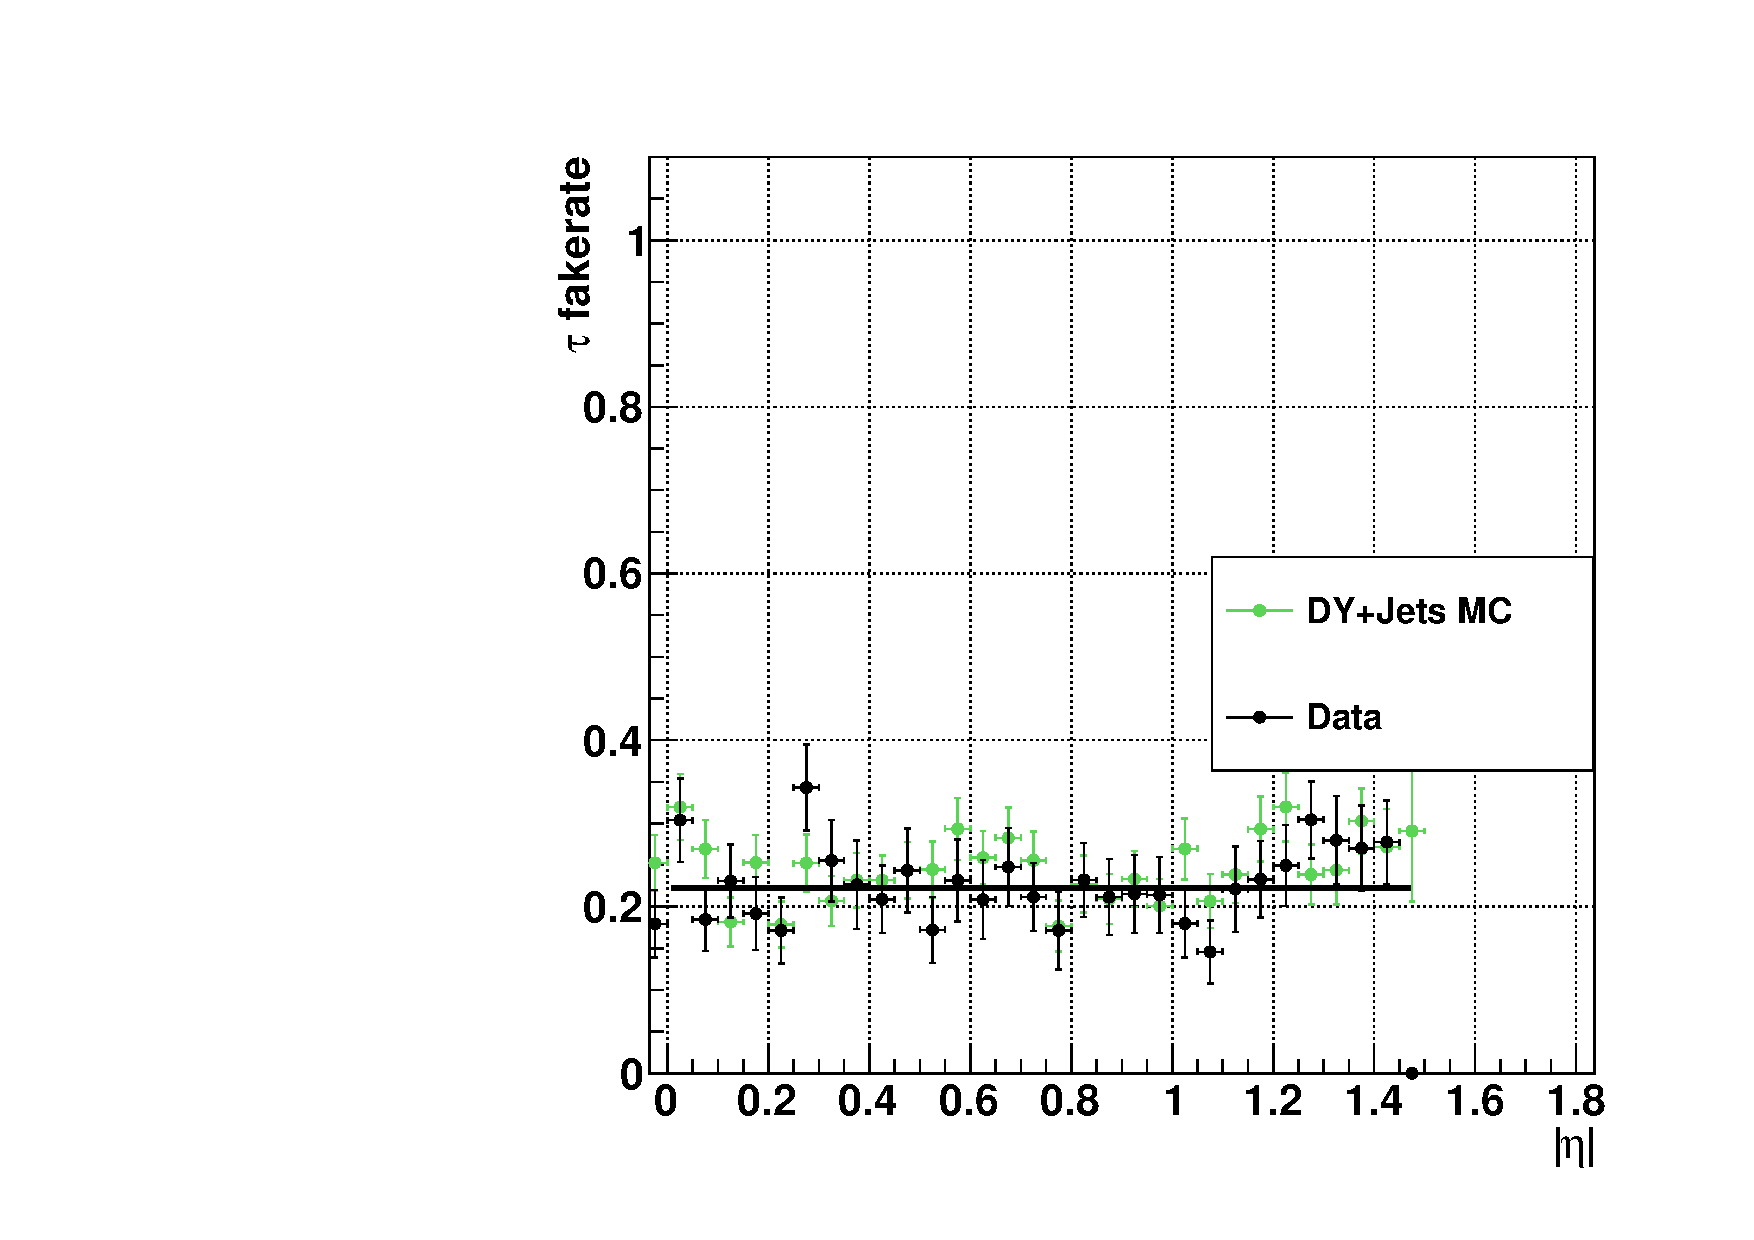
\includegraphics[width=0.3\textwidth]{chapterfakerate/preselectionDecay0EB_preselectionVLooseIsoDecay0EB_tEta_fakeRate.pdf}}
     \subfigure[tau decay mode 1 EB]{ 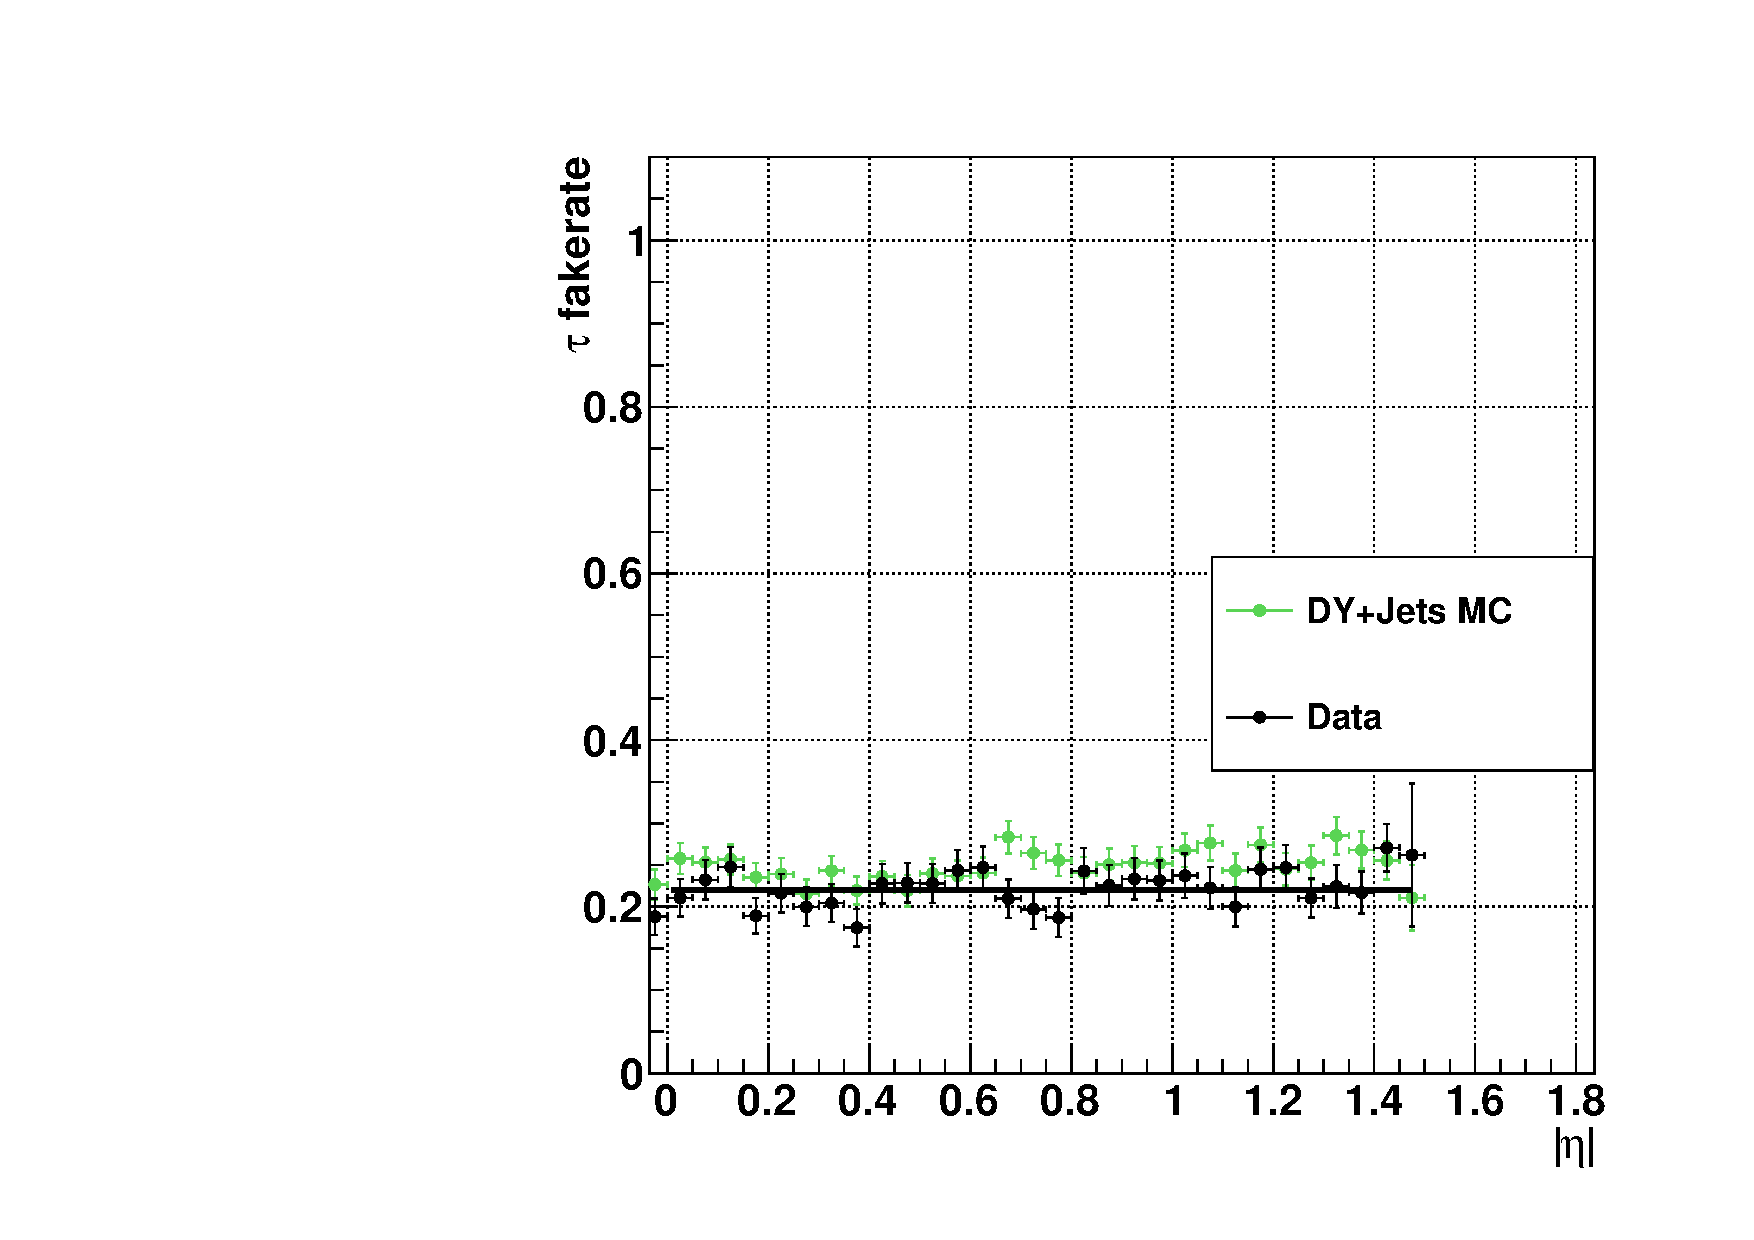
\includegraphics[width=0.3\textwidth]{chapterfakerate/preselectionDecay1EB_preselectionVLooseIsoDecay1EB_tEta_fakeRate.pdf}}
      \subfigure[tau decay mode 10 EB]{ 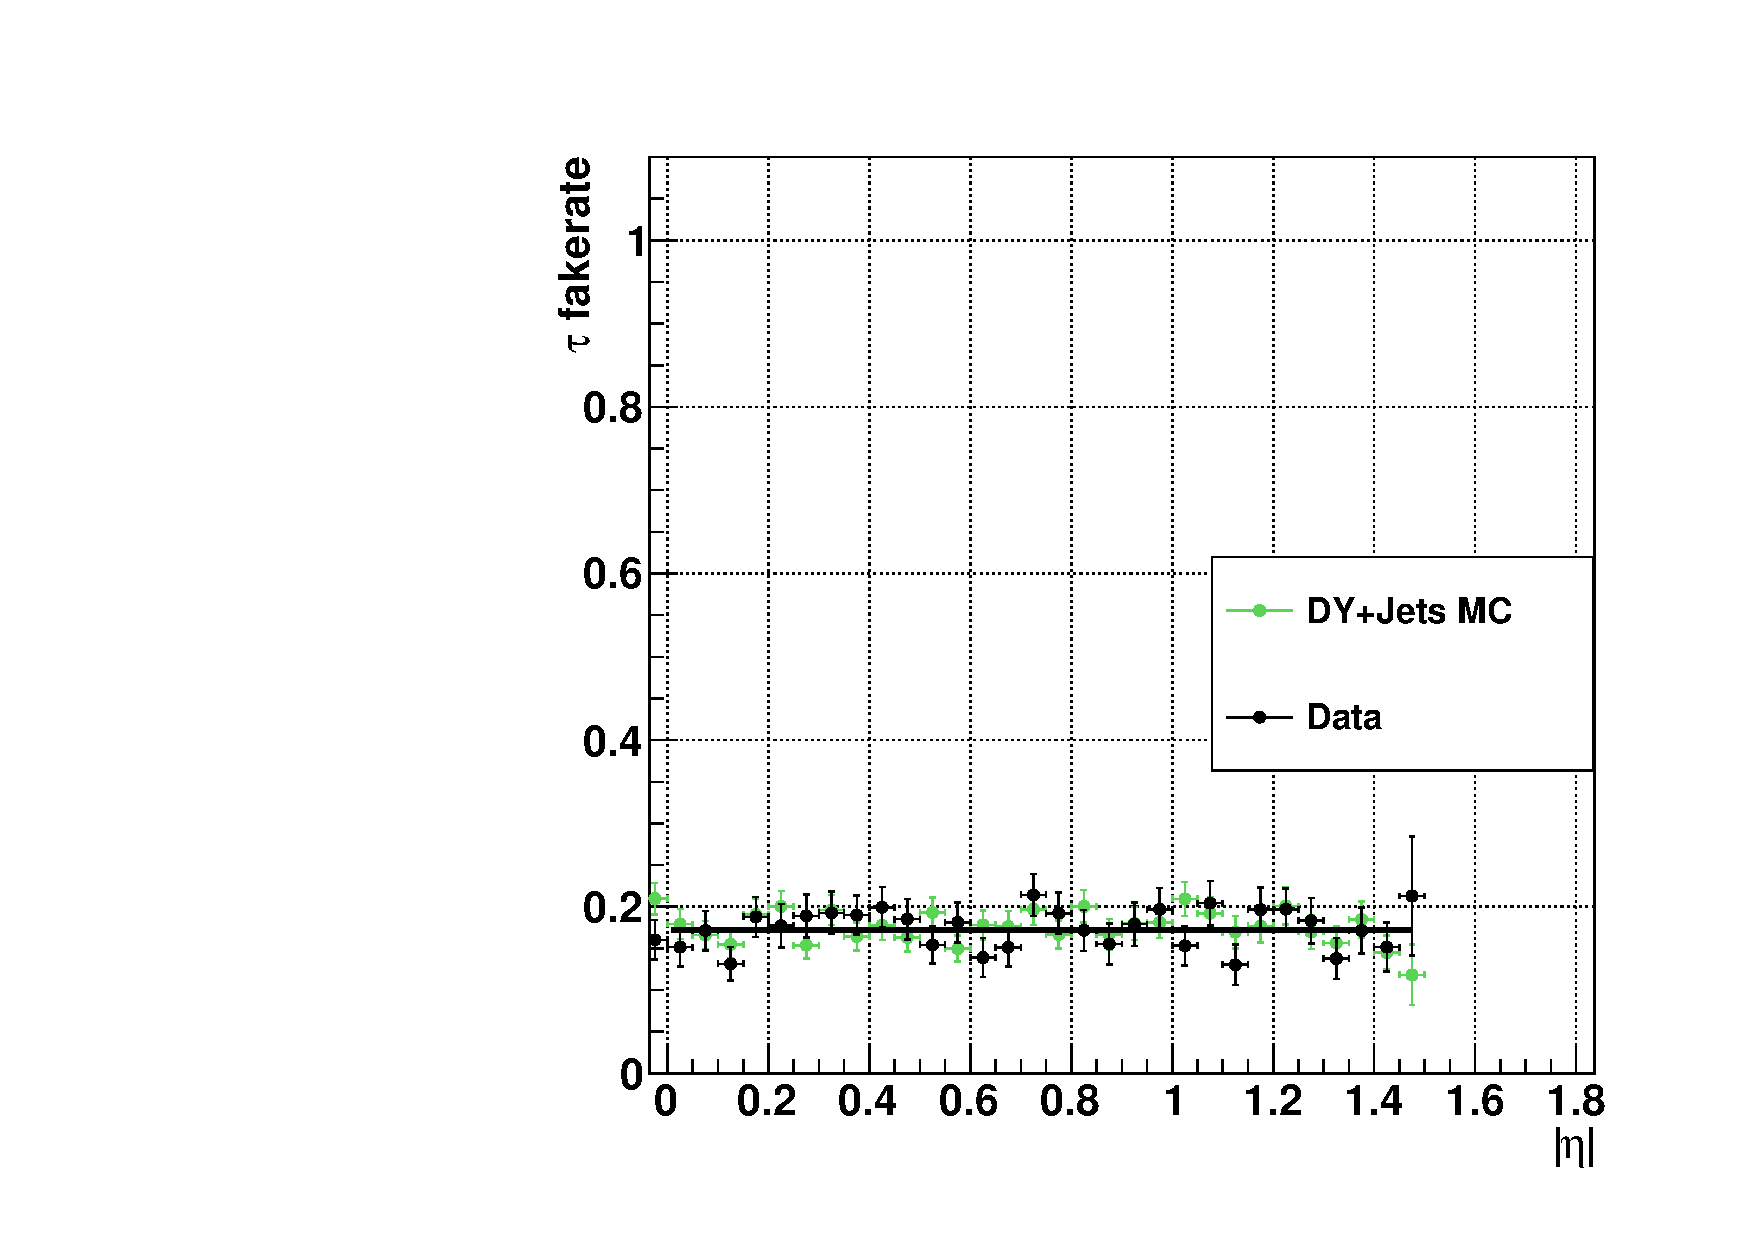
\includegraphics[width=0.3\textwidth]{chapterfakerate/preselectionDecay10EB_preselectionVLooseIsoDecay10EB_tEta_fakeRate.pdf}}\\
      \subfigure[tau decay mode 0 EE]{ 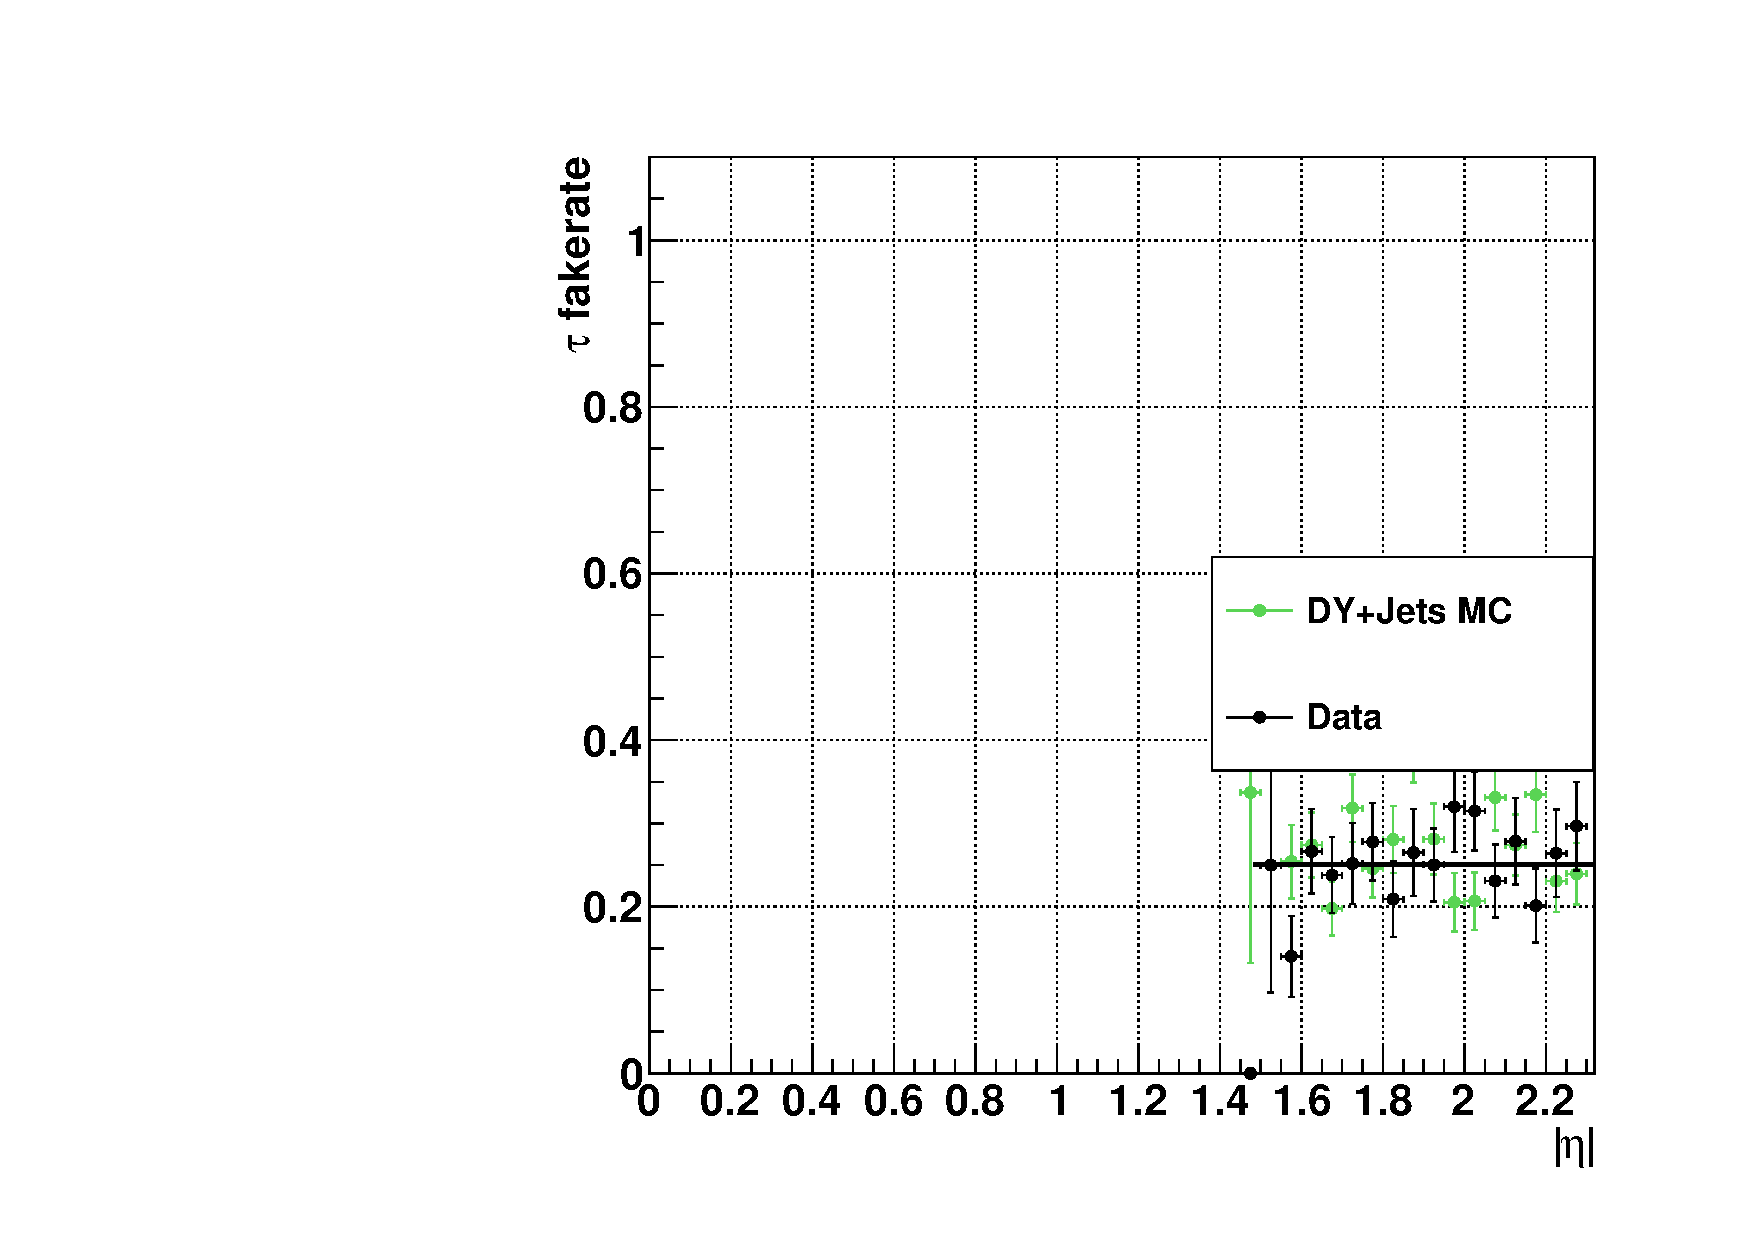
\includegraphics[width=0.3\textwidth]{chapterfakerate/preselectionDecay0EE_preselectionVLooseIsoDecay0EE_tEta_fakeRate.pdf}}
     \subfigure[tau decay mode 1 EE]{ 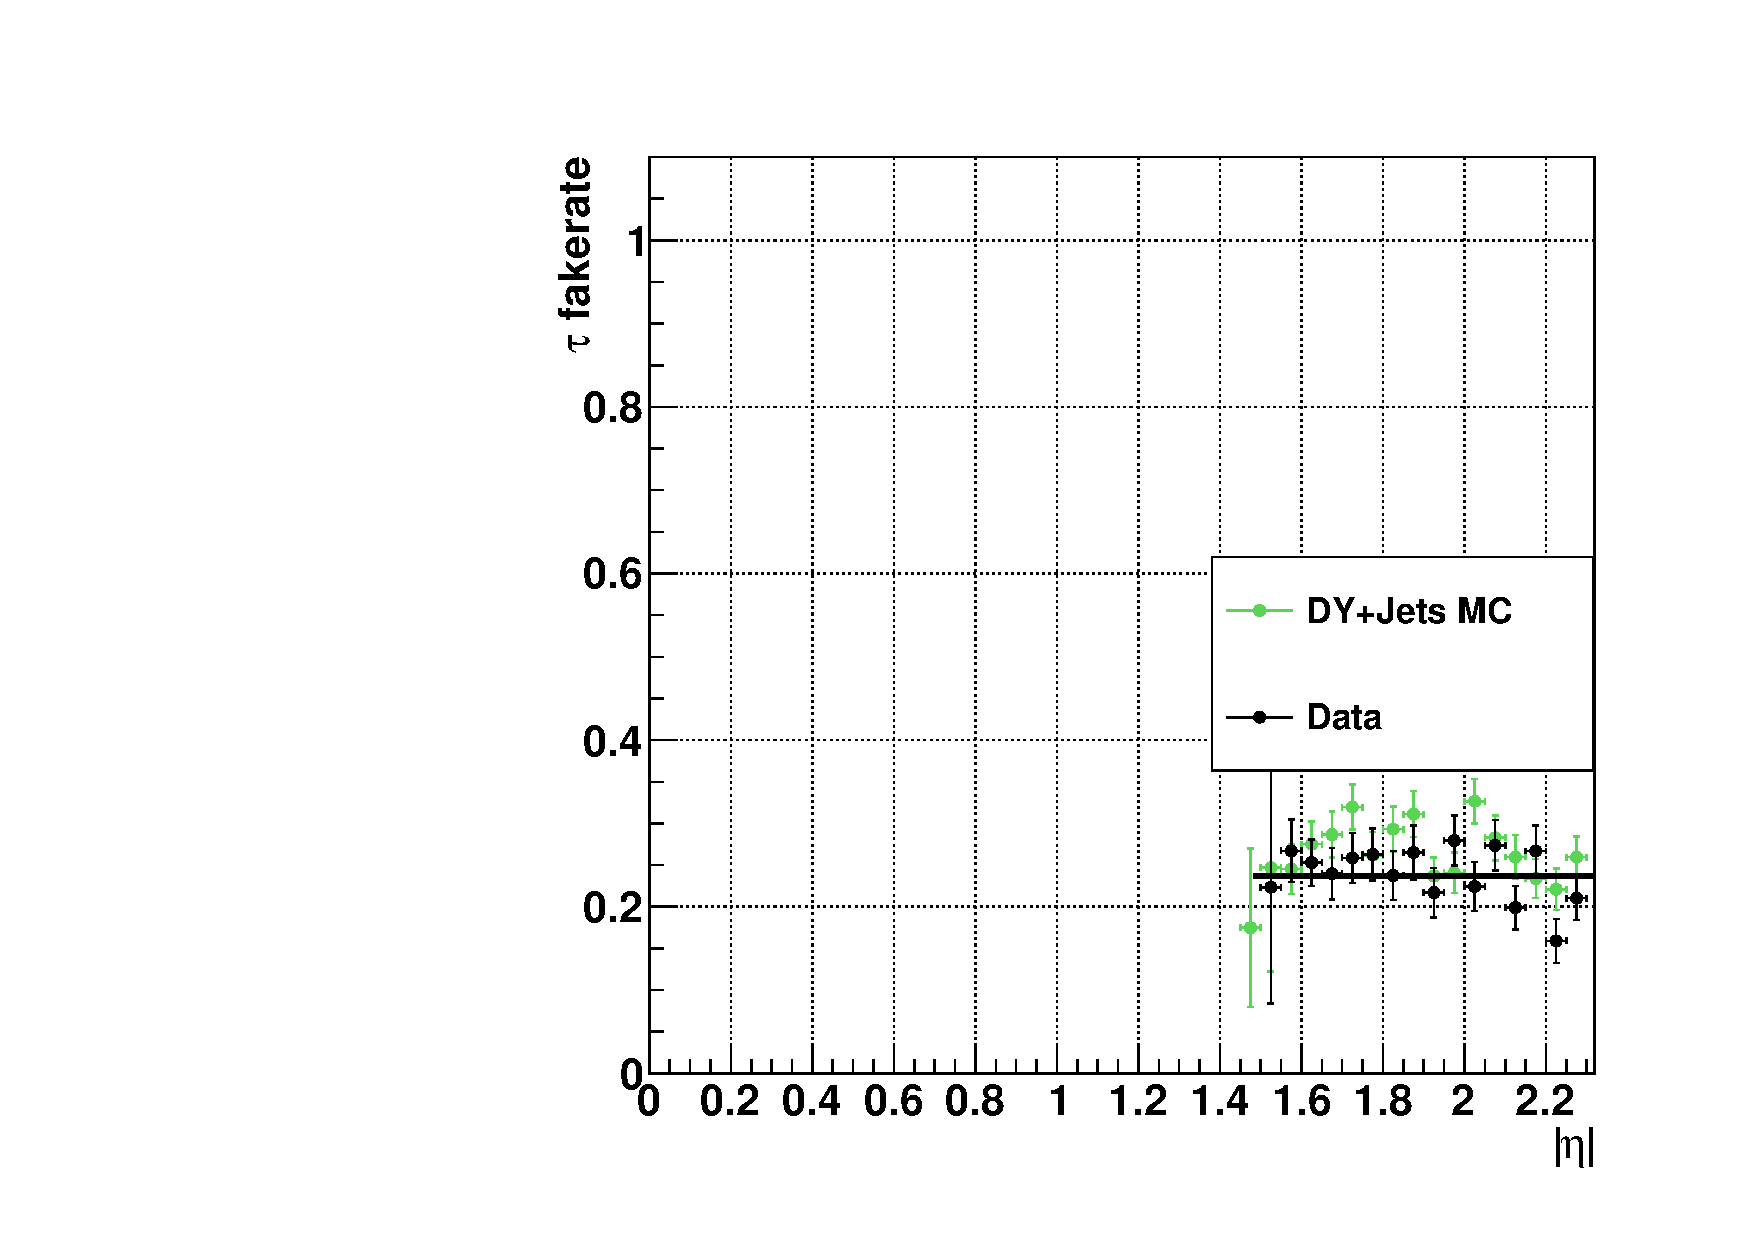
\includegraphics[width=0.3\textwidth]{chapterfakerate/preselectionDecay1EE_preselectionVLooseIsoDecay1EE_tEta_fakeRate.pdf}}
      \subfigure[tau decay mode 10 EE]{ 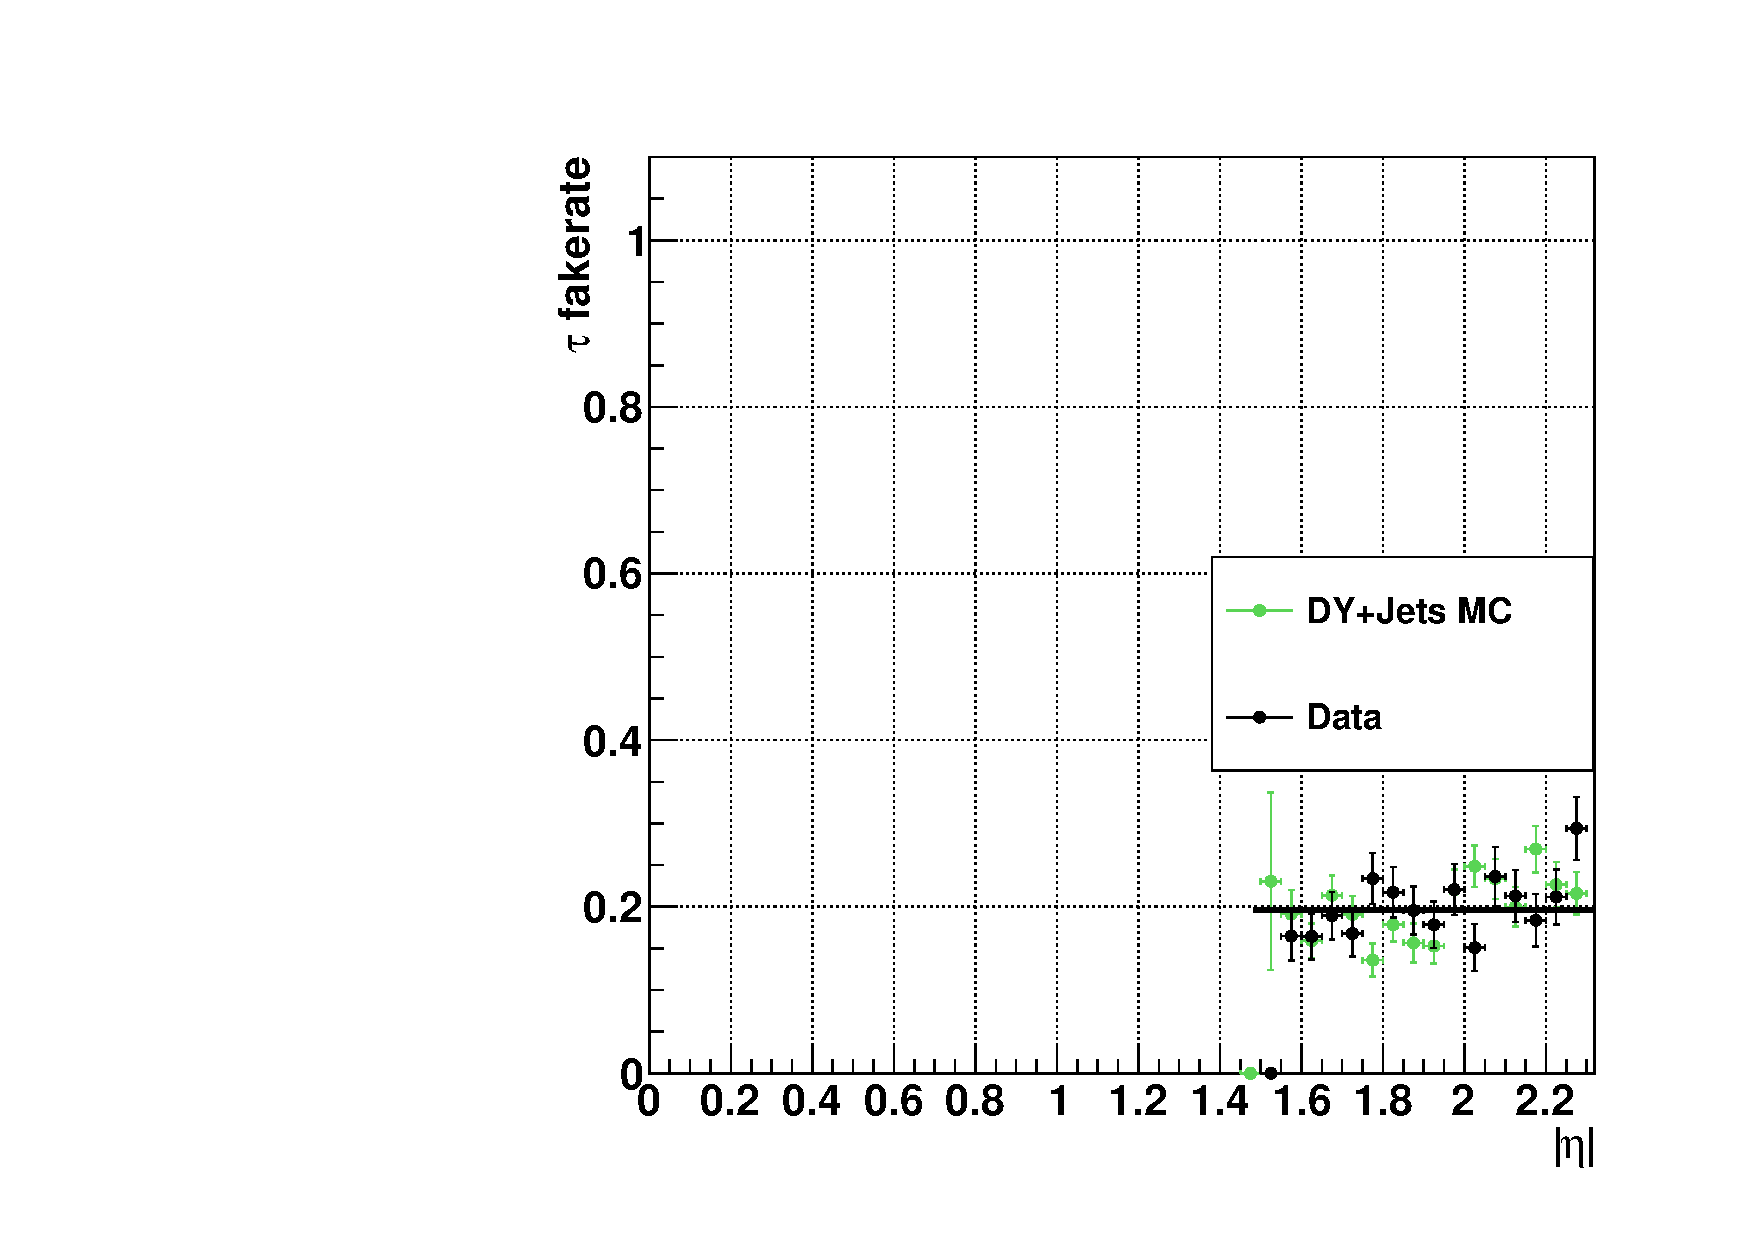
\includegraphics[width=0.3\textwidth]{chapterfakerate/preselectionDecay10EE_preselectionVLooseIsoDecay10EE_tEta_fakeRate.pdf}}\\
     \caption{$f_{\Pgt}$ ratio for the $\Pgt$ fake rate calculation shows in term of tau decay modes and $\eta$}
     \label{fig:fakerationumber}
\end{figure}

The misidentified muon events in the high mass LFV search are less than 5\% of the total misidentified events, so misidentified muon events are not considered. Study has been performed with Z+jets events, similar to the misidentified $\Pgt$ lepton study. As shown in Fig.~\ref{fig:MisidentifiedMuon}, in which the misidentified muons are added in and plotted separately with the misidentified $\Pgt$, compared with misidentified taus, misidentified muons are neglectable. 
 
\begin{figure}[htbp] 
\centering
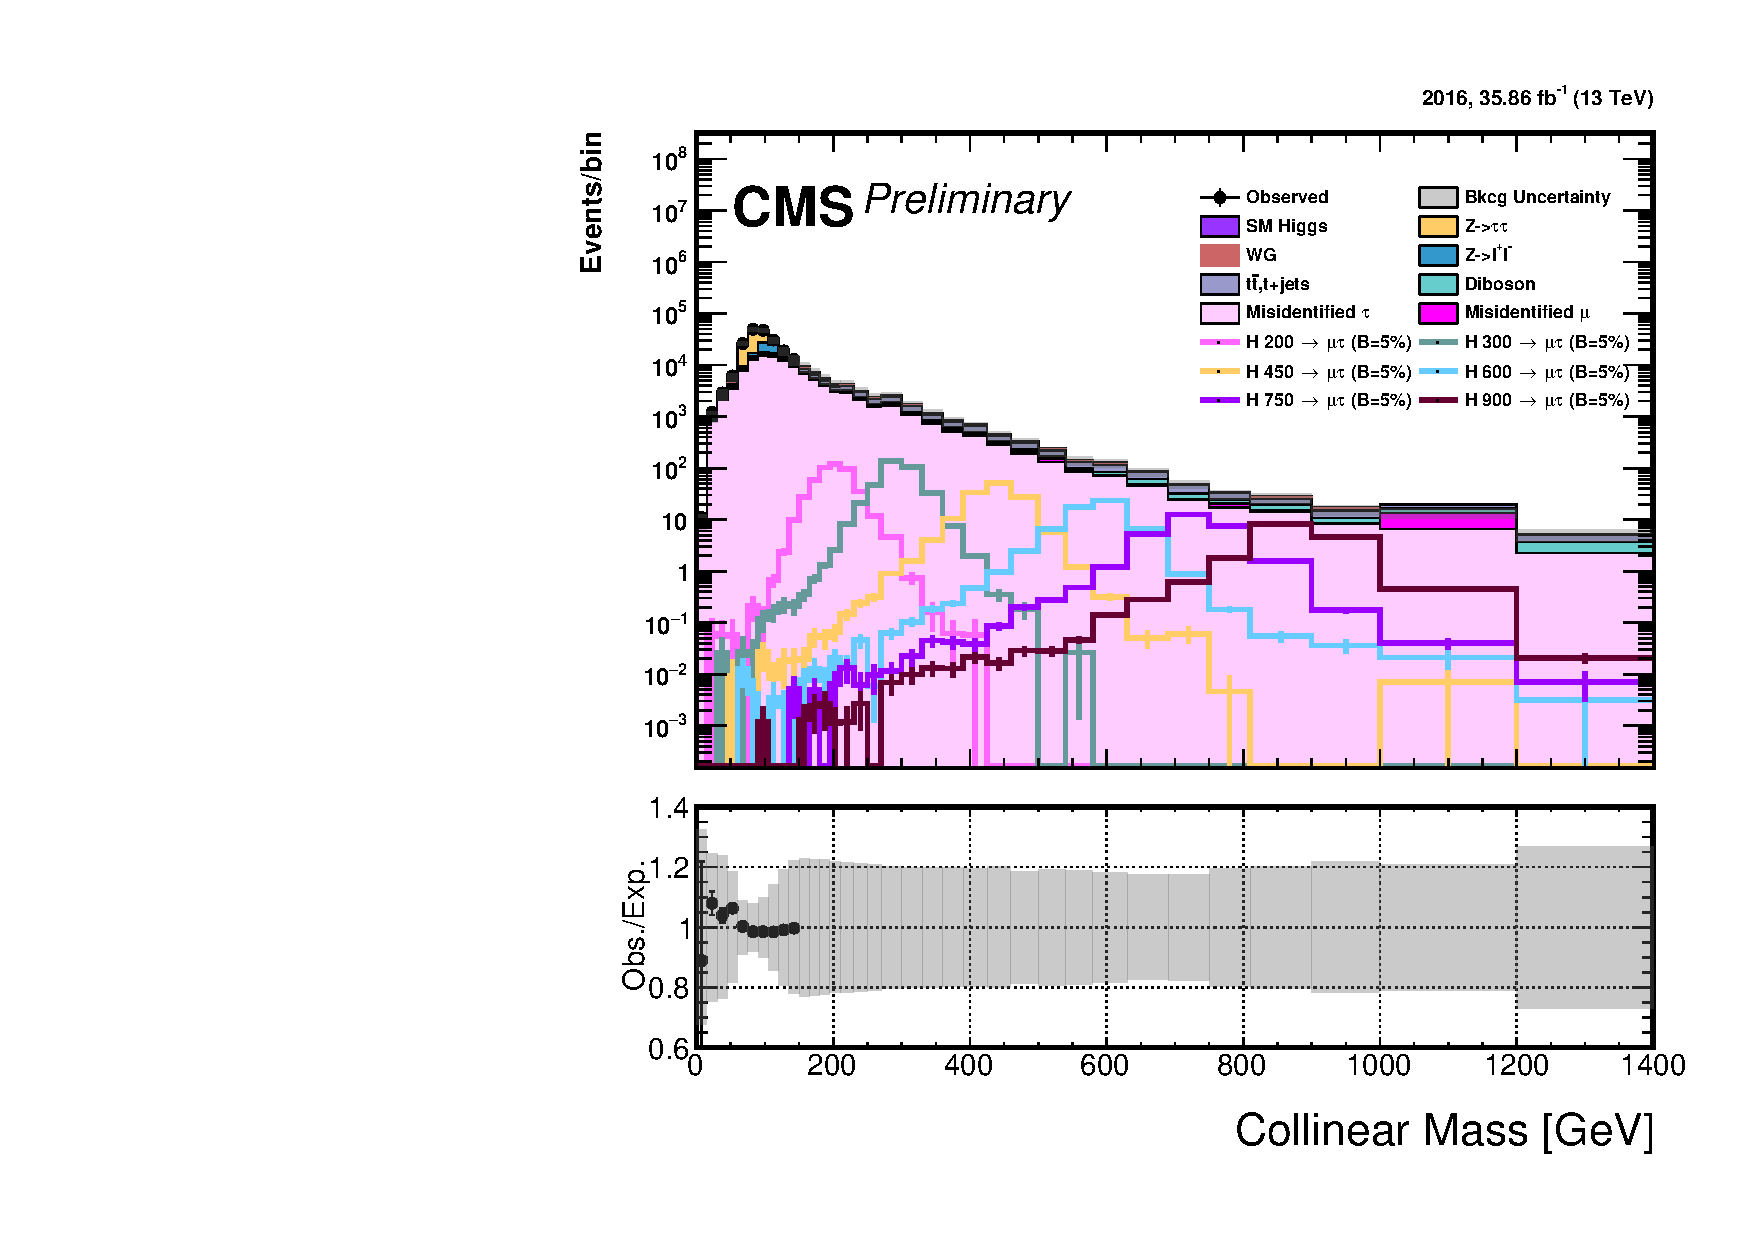
\includegraphics[width=0.6\textwidth]{chapterfakerate/LFV_preselection_collMass_type1_200Fakes_PoissonErrorsMuonfake.pdf}
\caption{Base selection $M_{col}$ distribution with misidentified muons added .}
\label{fig:MisidentifiedMuon}
\end{figure}

The validation of the misidentified lepton background with full data driven method is performed in a like-sign sample and W+jets enriched control region. In $\Hmuhad$ channel, the like-sign sample validation requires the events pass the loose selection, the same as the signal region, but with inverted charge. Misidentified background is enriched with the requirement of inverting charge. In the W+jets enriched control region, events that pass the loose selection are further selected with  $M_T(\Pgt)>60$ GeV and $M_T(\Pgm)>80$ GeV.  In both of the control regions, misidentified background is the dominant one, as shown in Fig.~\ref{fig:fakebackgroundValidation}. With full data driven method, applied with the $\Pgt(f_{\Pgt})$ as weight, the like-sign and W+jets control regions show good data and MC agreement. 


\begin{figure}[htbp] 
     \centering
     \subfigure[Wjets enriched control region]{ 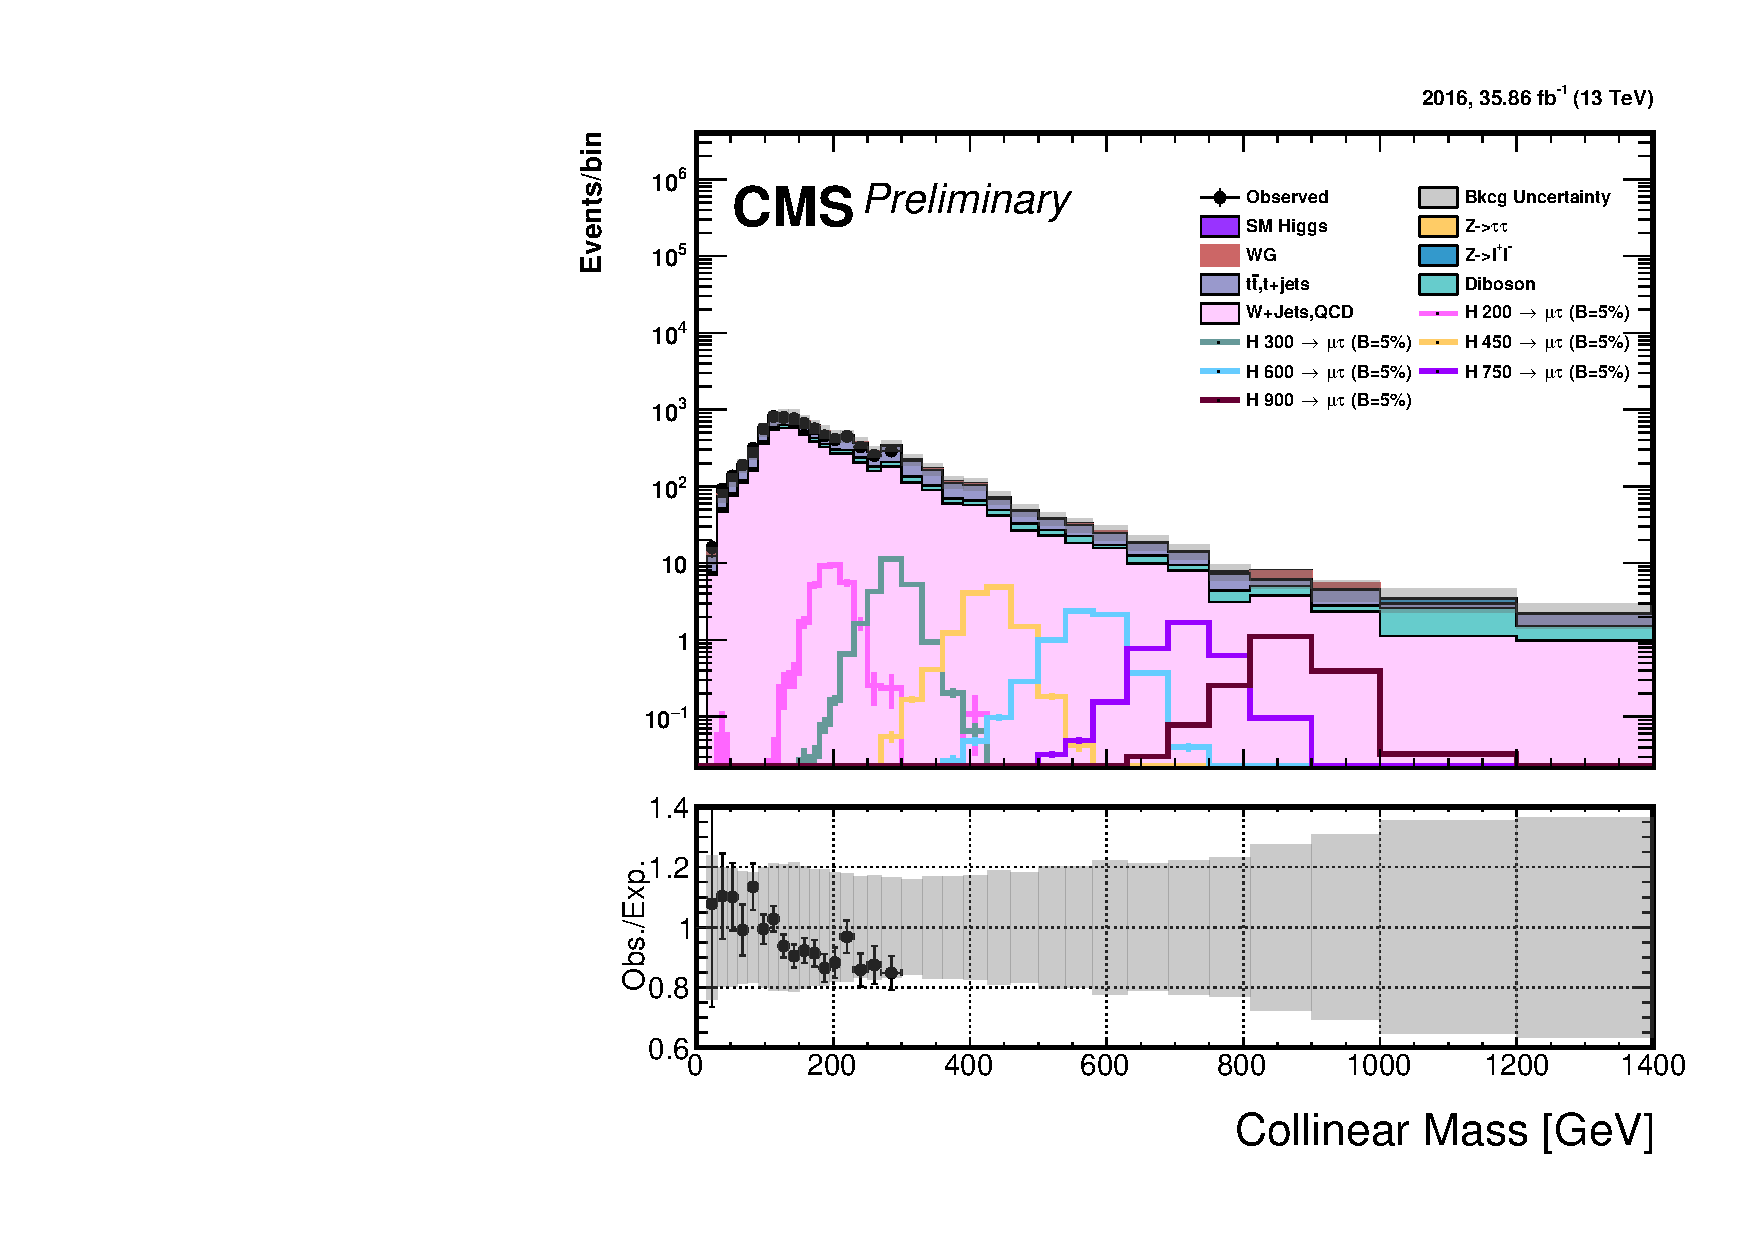
\includegraphics[width=0.4\textwidth]{chapterfakerate/LFV_preslectionEnWjets_collMass_type1_200Fakes_PoissonErrors.pdf}}
     \subfigure[Like-sign control region]{ 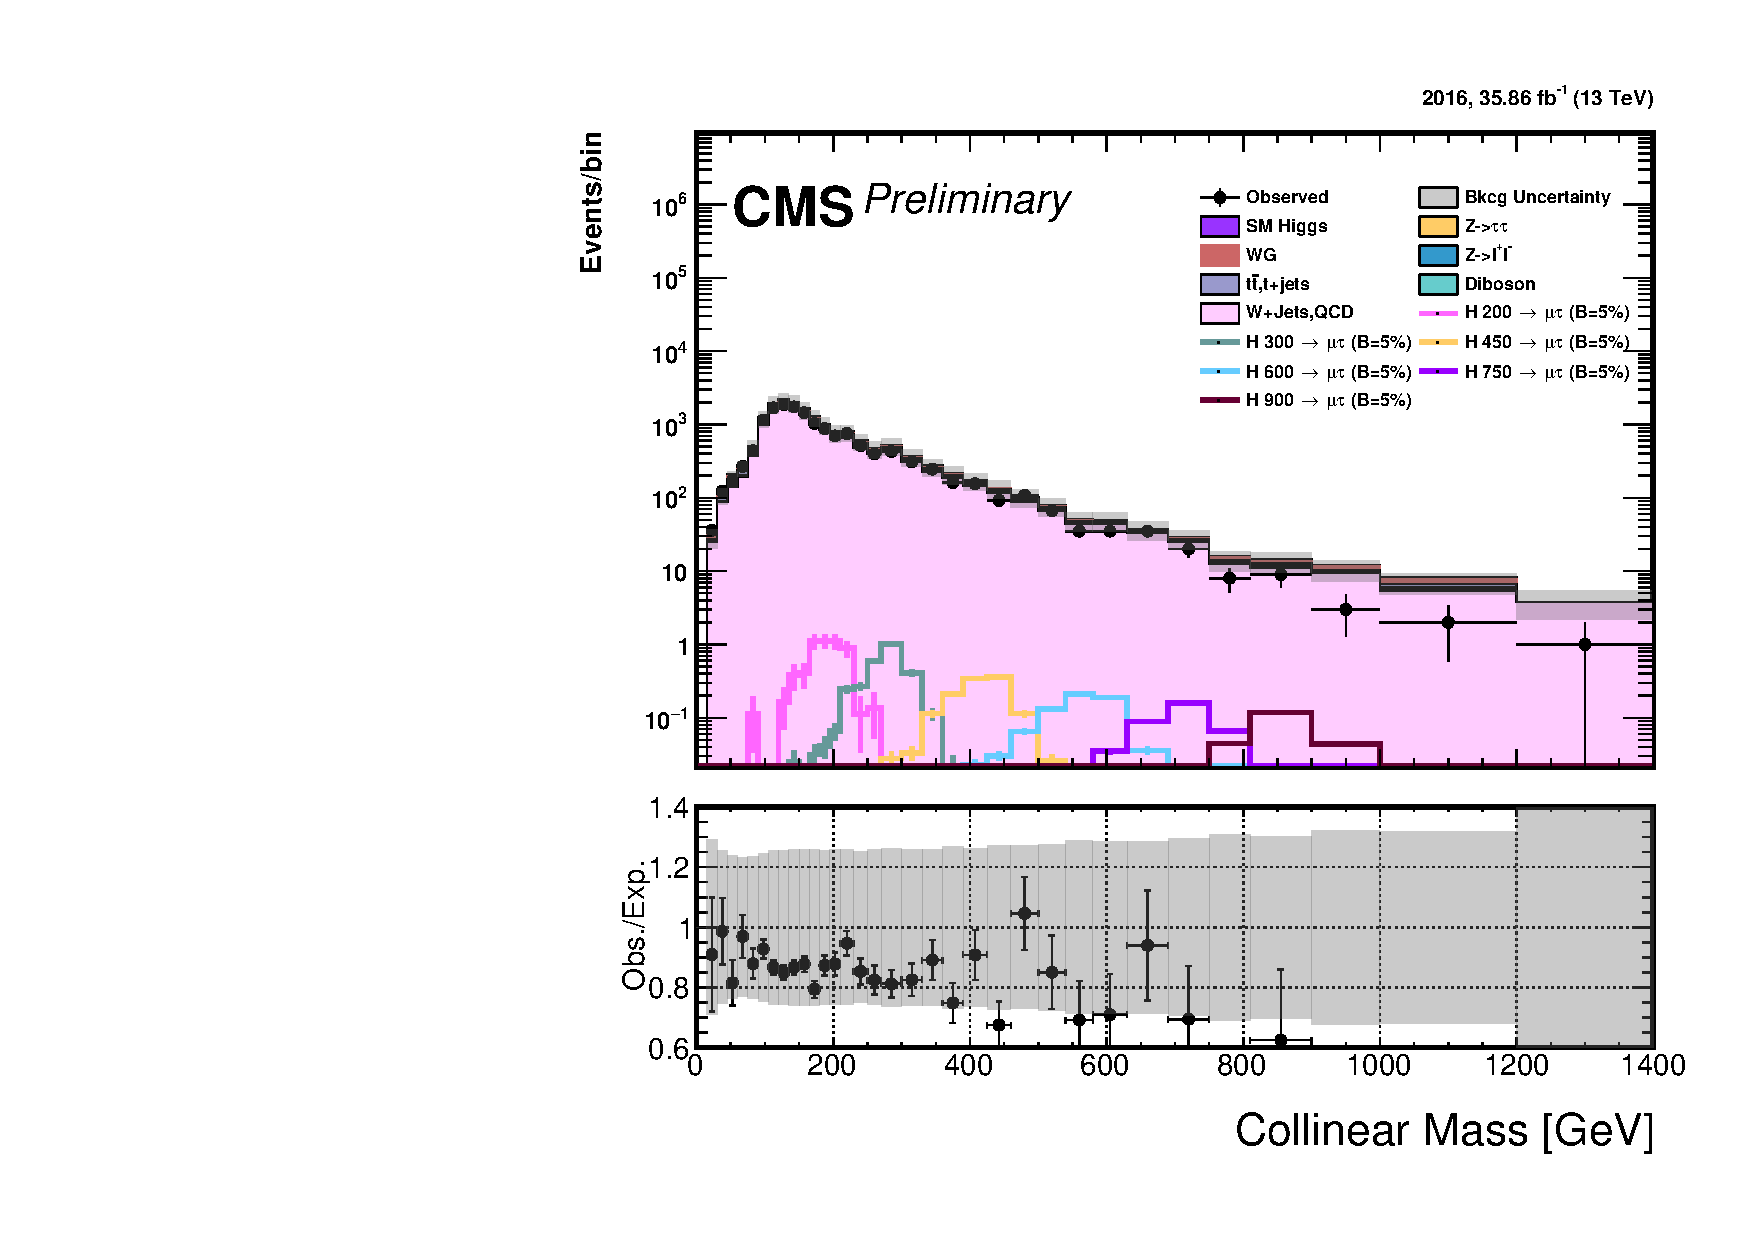
\includegraphics[width=0.4\textwidth]{chapterfakerate/LFV_preselectionSS_collMass_type1_200Fakes_PoissonErrors.pdf}}
     \caption{The validation of full data driven method for the misidentified lepton background. 30\% of uncertainty is assumed in both cases. }
     \label{fig:fakebackgroundValidation}
\end{figure}











\subsection{Event selection}
In 13 TeV $H\rightarrow\Pgm\Pgt_h$ analyses, events are selected in several steps. A loose selection selects on the different IDs, energy, geometry parameters of the analysis related objects and followed by a tighter set of selection criteria in which selection requirements are placed on the kinematics variables and fits on variable $\mcol$. This selection sequence is referred as $\mcol$ fit analysis.

\subsection{Base selection}
Tau leptons from signal events decay hadronically. SM higgs is much heavier than its decay products $\Pgm$ and $\Pgt$. $\Pgm$ and $\Pgt$ leptons are expected to have high $P_{T}$. The decay products from signal events are boosted, a cut on $\Delta R=\sqrt(\Delta phi^{2}+\Delta eta^{2})$, $\Delta R>0.3$ is applied. $\Pgm$ and $\Pgt$ candidates are required to have opposite sign of charges as Higgs has no electric charge. Further, events with additional $\Pgm$ and $\Pgt$ that pass a loose selection, events with jets that are identified by the combined secondary vertex(CSVv2) b-tagging algorithm \cite{btag_ago} as a b quark jets are discarded. Trigger HLT\_Mu50 or HLT\_TkMu50 used in the analysis selects isolated muons that have energy higher than 50 GeV at HLT level. An further $P_{T}$ cut on reconstructed $\Pgm$,  $P_{T}>53$ GeV and $|\eta|<2.4$ are required. Muons are required to pass the recommended Medium muon ID and tight cut based isolation $I^{\Pgm}_{rel}<0.15$. 
Hadronic taus are required to have $P_T>30$ GeV,$|\eta|<2.3$, passing old tau decay mode finding, the MVA based tight tau isolation ID and tau discriminators against electrons and muons. 

Events in the analysis are divided into two categories based on the number of jets. Gluon gluon fusion Higgs production is the only production channel considered in this analysis. In 0 jet category, no events have jets pass the loose PF ID and  with jet $P_T>30$ GeV, $|\eta|<4.7$. In 1 jet category, events are required to have one jet passes losse PF ID and jet $P_T>30$ GeV, $|\eta|<4.7$.


\subsection{$\mcol$ fit analysis}
After the loose selection and the categorization, a further cut-based selection is applied. Variables that can help distinguish signal from background are $P_{T}^{\Pgm}$, $P_{T}^{\Pgt}$ and $M_{T}(\Pgt_{h})$.
The cut-based selection are performed in two mass ranges of high mass Higgs search. Low mass range includes high mass Higgs with mass 200 and 300 GeV. High mass range includes mass pints 450, 600, 750 and 900 GeV.   


 The lepton $P_{T}$ variables are very powerful background discriminant variables. Leptons from signal process incline to have higher $P_{T}$ values, by cutting tighter on the lepton $P_{T}$, more background events can be removed. Boosted neutrino from $\Pgt$ decay in the signal events contribute to MET which renders $M_{T}(\Pgt_{h})$ distinguishing power between signal and backgounds. Optimization is proceeded with only Monte Carlo samples so as not to double use data. In $\Hmuhad$  channel, the misidentified background in the optimization is estimated by semi-data driven method. Cuts have been optimized to have the most stringent expected limits. If looser values of the cuts give the same expected limits as the tighter ones, then the looser cut values are chosen to have more statistics. Examples of optimization by checking the limits are shown in Figure. \ref{fig:optMThighmass}. A full summary of the cuts optimized for $\Hmuhad$ is shown in Table.~\ref{tab:Mhadcategories}


\begin{figure}[htbp] 
     \centering
     \subfigure[Low mass range 0 jet $\pt^{\Pgm}$]{ 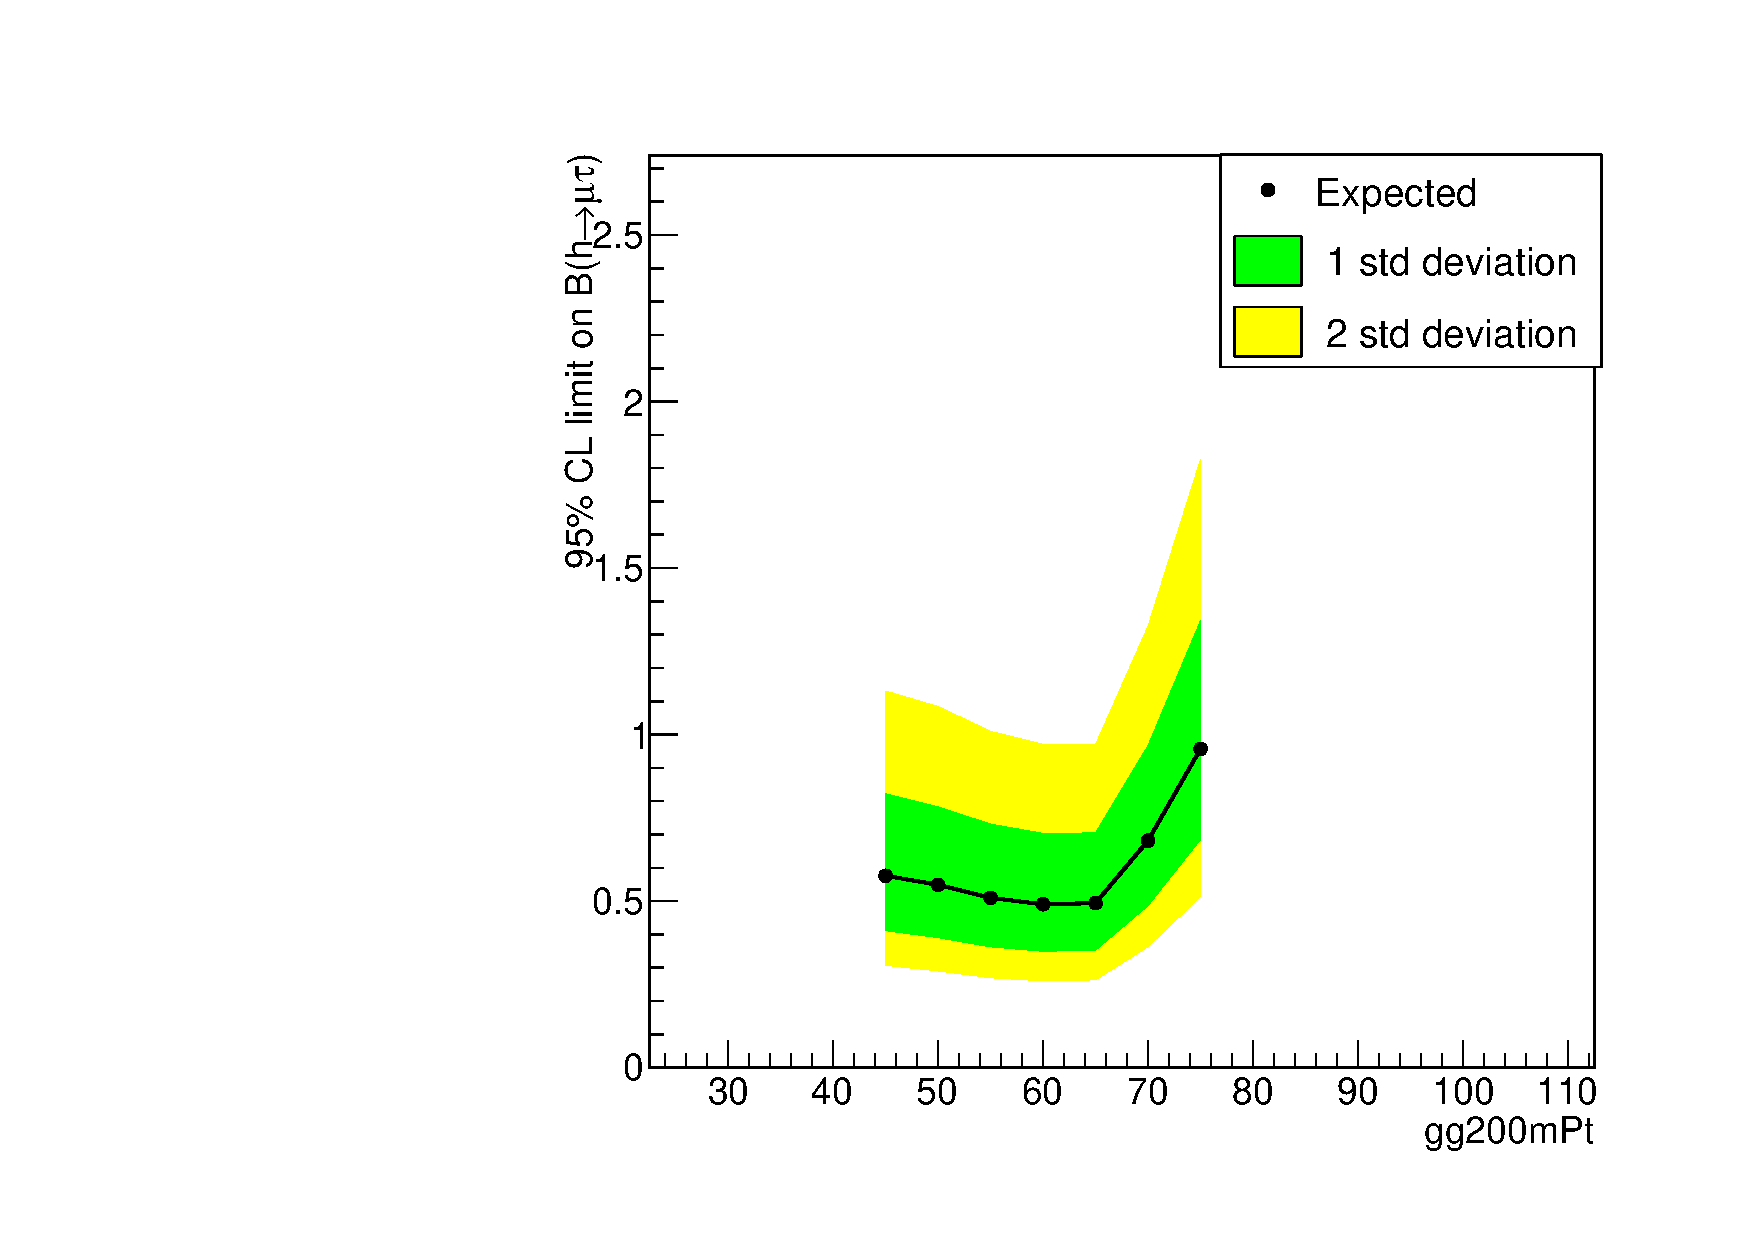
\includegraphics[width=0.4\textwidth]{chapterfakerate/Tuning/gg200mPt.pdf}}
     \subfigure[Low mass range 0 jet $\pt^{\Pgt}$]{ 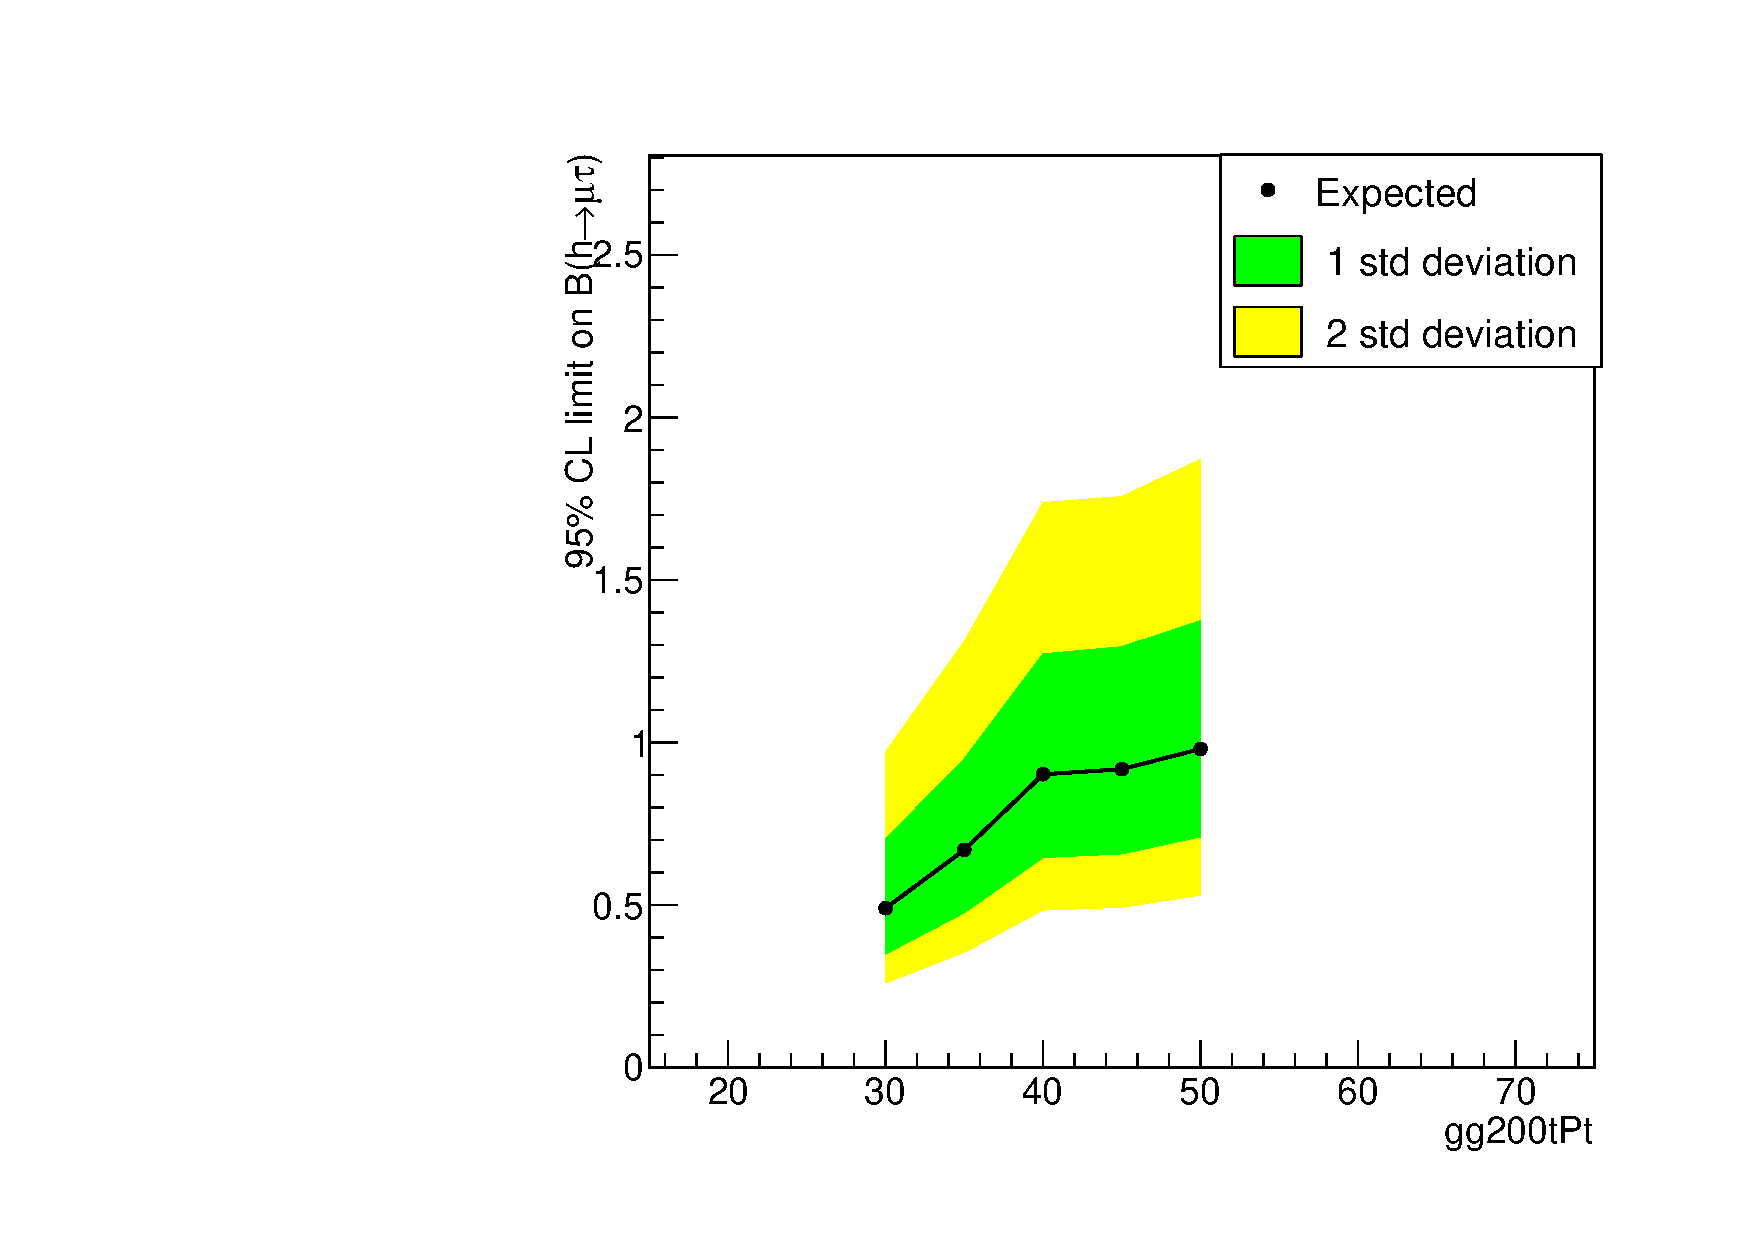
\includegraphics[width=0.4\textwidth]{chapterfakerate/Tuning/gg200tPt.pdf}}\\
     \subfigure[Low mass range 0 jet $M_{T}(\Pgt_{h})$]{ 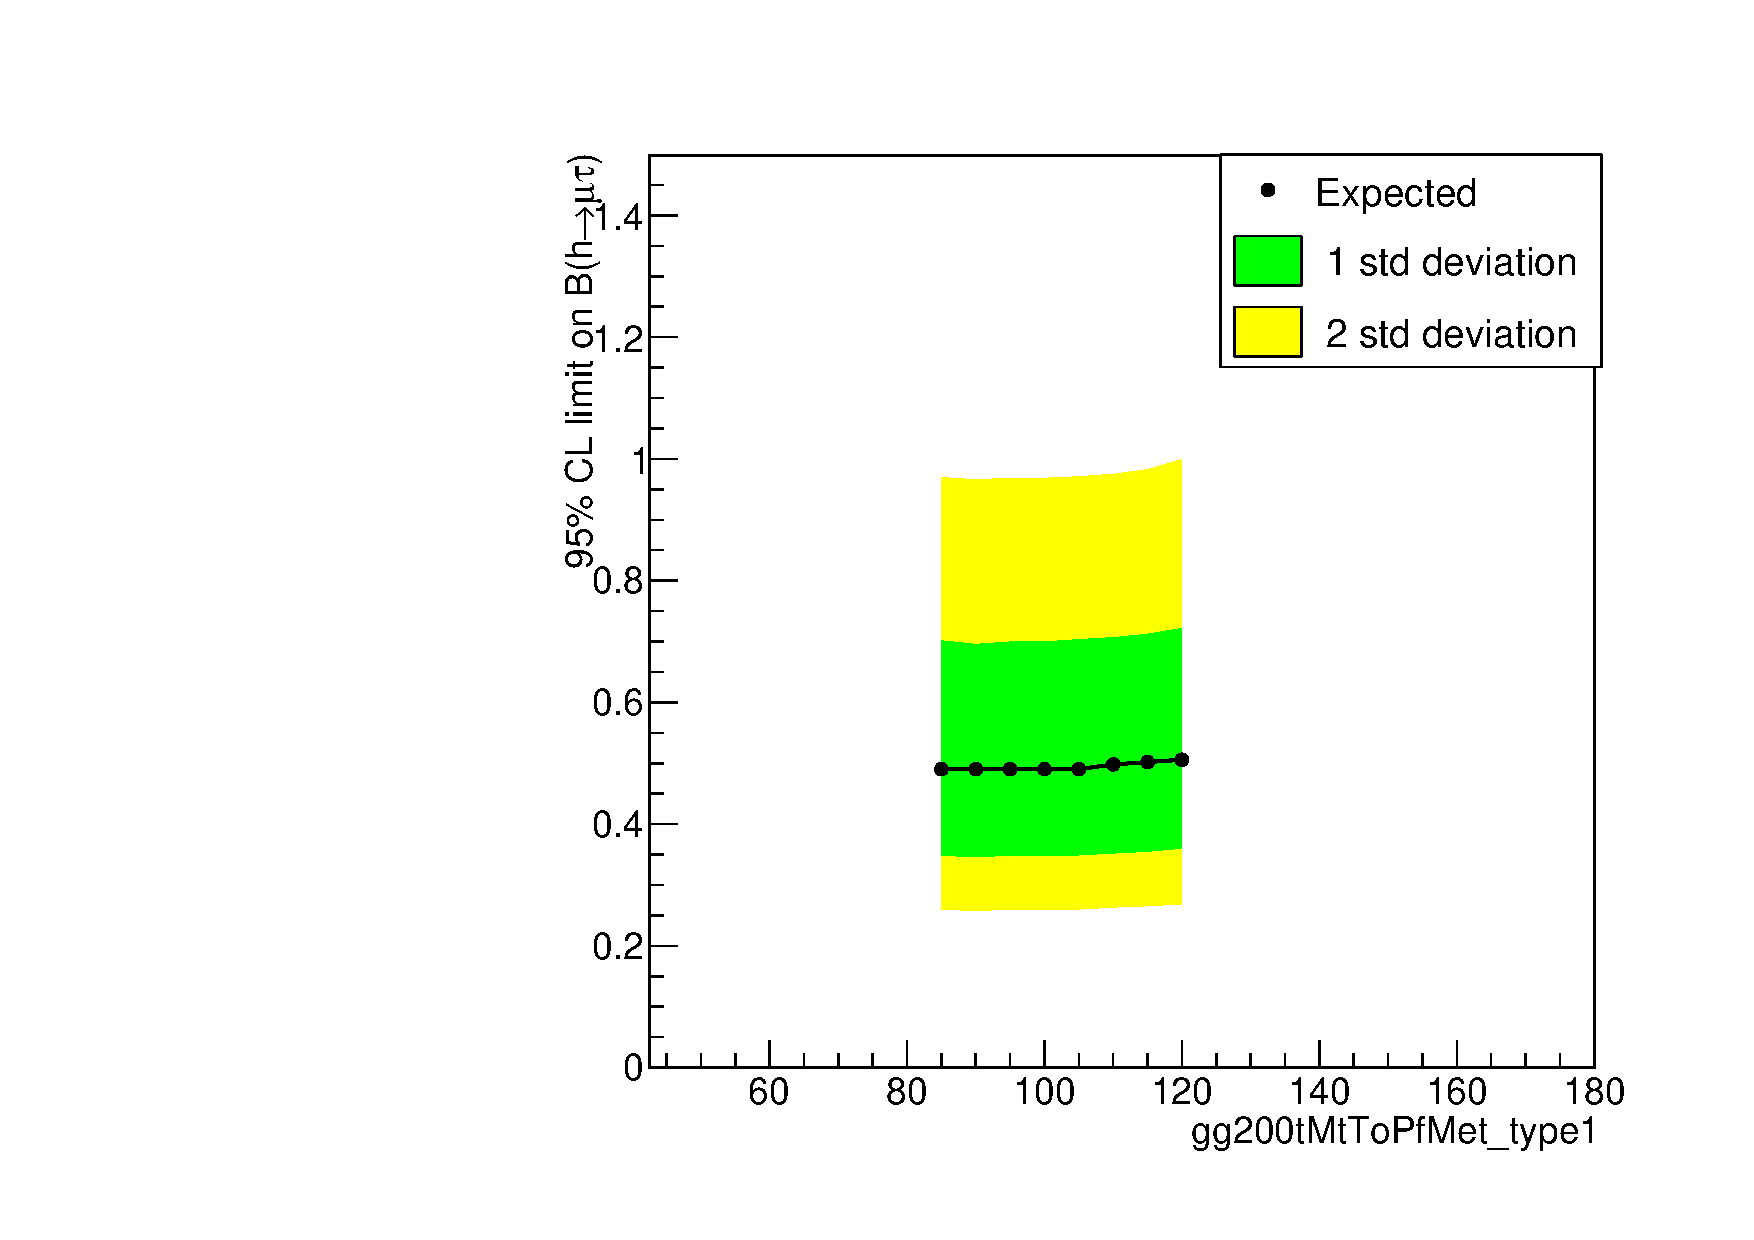
\includegraphics[width=0.4\textwidth]{chapterfakerate/Tuning/gg200tMtToPfMet_type1.pdf}}
     \subfigure[High mass range 1 jet $\pt^{\Pgm}$]{ 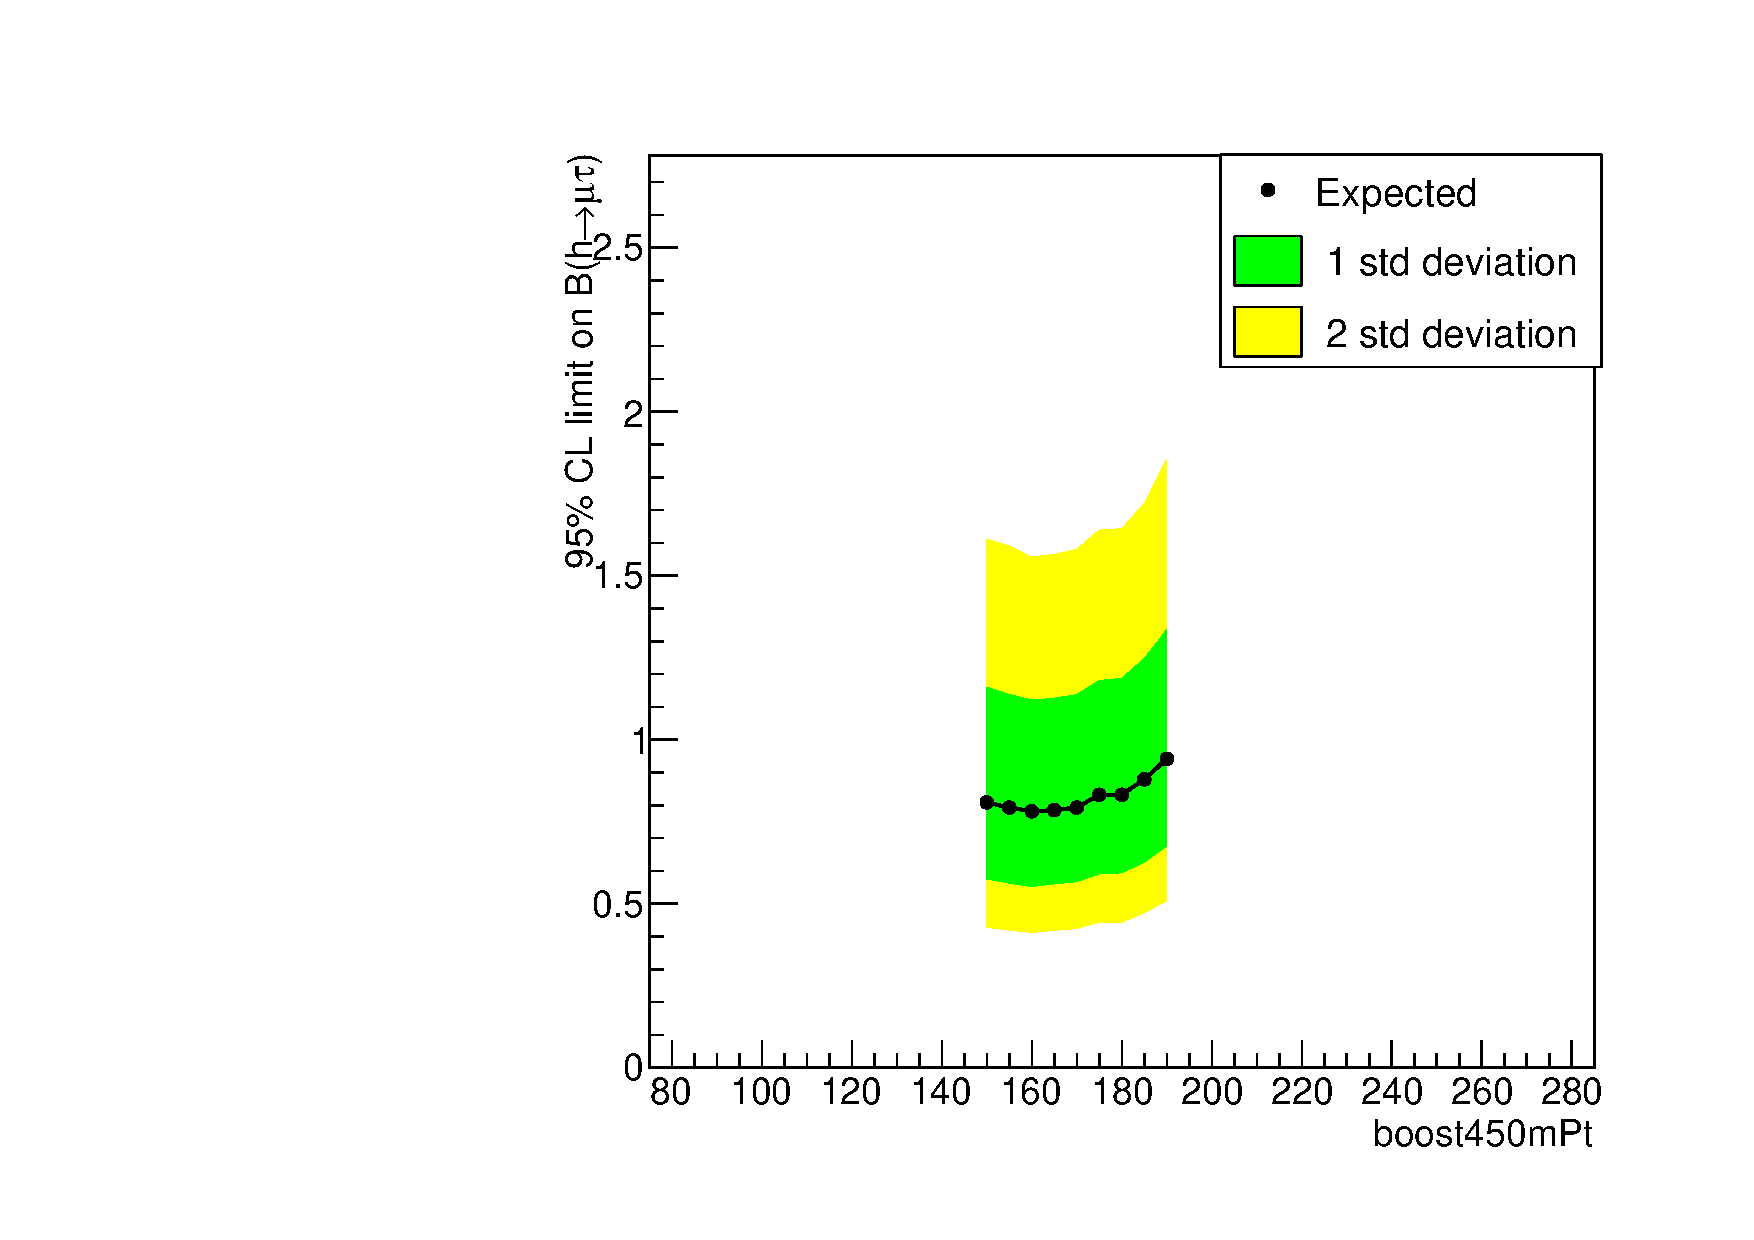
\includegraphics[width=0.4\textwidth]{chapterfakerate/Tuning/boost450mPt.pdf}}
     \subfigure[High mass range 1 jet $\pt^{\Pgt}$]{ 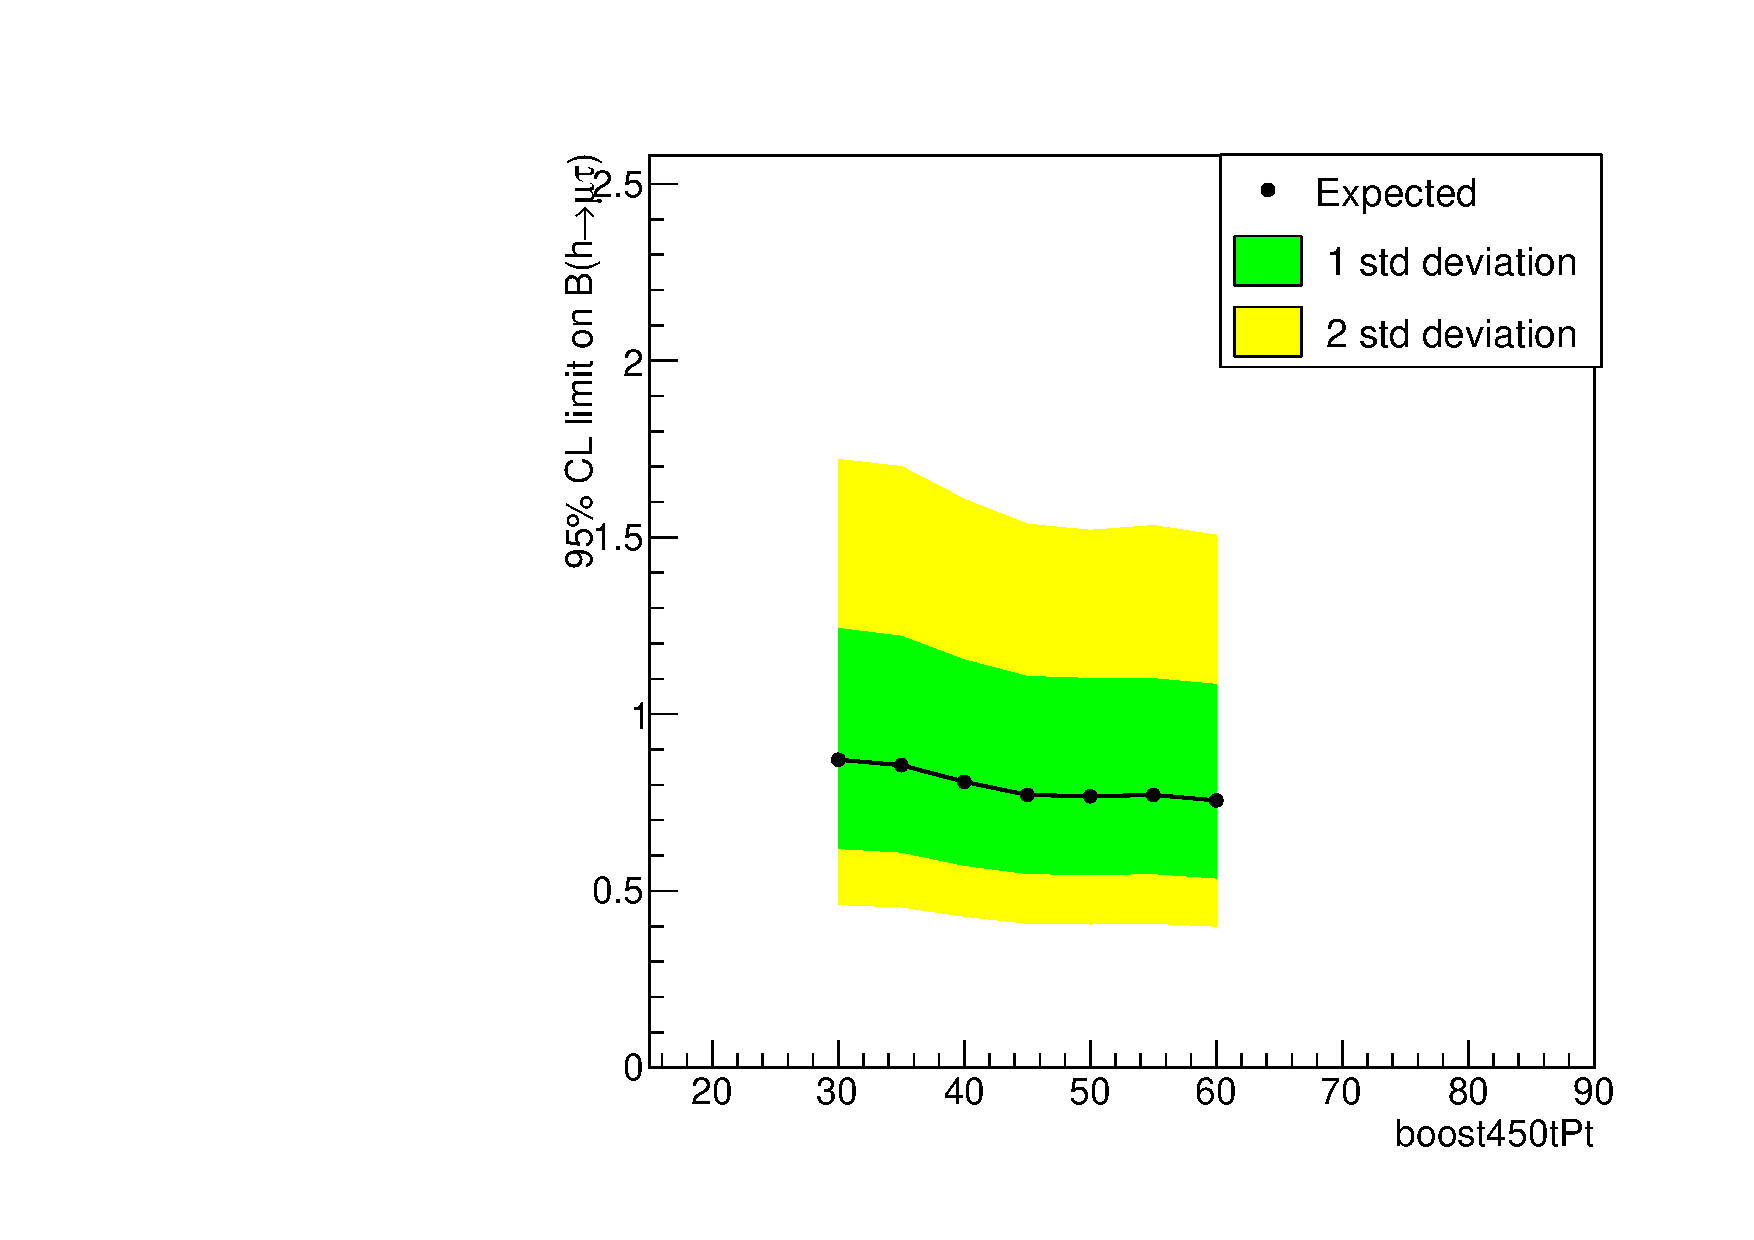
\includegraphics[width=0.4\textwidth]{chapterfakerate/Tuning/boost450tPt.pdf}}
     \subfigure[High mass range 1 jet $M_{T}(\Pgt_{h})$]{ 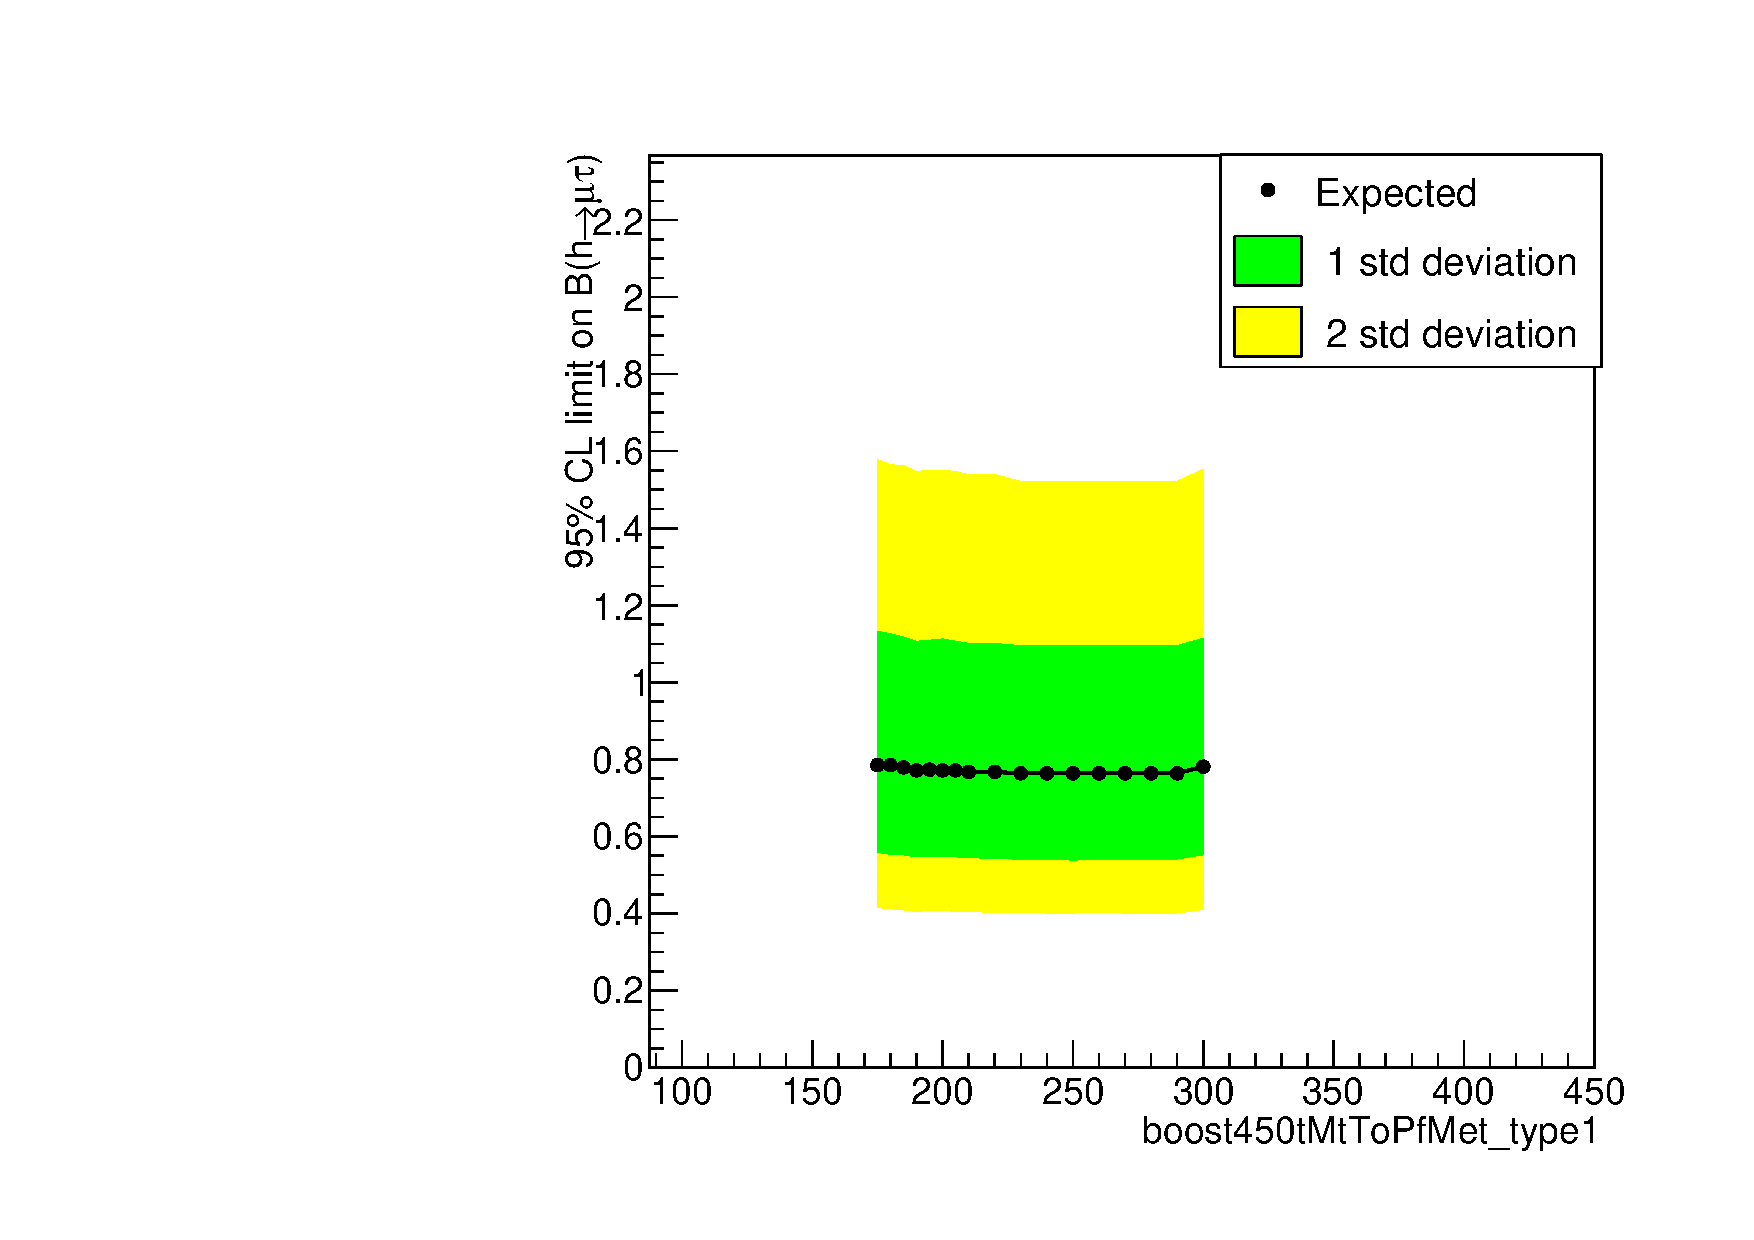
\includegraphics[width=0.4\textwidth]{chapterfakerate/Tuning/boost450tMtToPfMet_type1.pdf}}
     \caption{Examples of optimization with expected limits in low mass range 0 jet and high mass range 1 jet.}
     \label{fig:optMThighmass}
\end{figure}



\begin{table}[hbtp]
  \begin{center}
  \caption{Selection criteria in each category with the optimization of the $\Hmuhad$ analysis}
  \begin{tabular}{l} \hline
  {\bf Low mass range 0-jet category} \\ \hline
  \tabitem $\pt^{\Pgm}>60$ GeV, $\pt^{\Pgt}>30$ GeV\\
  \tabitem $M_T(\Pgt)<105$ GeV \\
  \tabitem No jets with $\pt^{jet}>30$ GeV, $|\eta|<4.7$, LooseID \\ \hline
 {\bf Low mass range 1-jet category} \\ \hline
  \tabitem $\pt^{\Pgm}>60$ GeV, $\pt^{\Pgt}>30$ GeV \\
  \tabitem $M_T(\Pgt)<120$ GeV \\
  \tabitem One jet  with $\pt^{jet}>30$ GeV, $|\eta|<4.7$, LooseID
  \\ \hline
  {\bf High mass range 0-jet category} \\ \hline
  \tabitem $\pt^{\Pgm}>165$ GeV, $\pt^{\Pgt}>45$ GeV \\
  \tabitem $M_T(\Pgt)<200$ GeV \\\hline
  {\bf High mass range 1-jet category} \\ \hline
  \tabitem $\pt^{\Pgm}>165$ GeV, $\pt^{\Pgt}>45$ GeV \\
  \tabitem $M_T(\Pgt)<230$ GeV \\
   \tabitem One jet  with $\pt^{jet}>30$ GeV, $|\eta|<4.7$, LooseID  \\\hline
  \label{tab:Mhadcategories}
\end{tabular}
\end{center}
\end{table}







